\documentclass[isrm2, tisk]{fmfdelo}
\usepackage[utf8]{inputenc}
\usepackage[T1]{fontenc}
\usepackage[a-2b]{pdfx}
% Če pobrišete možnost tisk, bodo povezave obarvane,
% na začetku pa ne bo praznih strani po naslovu, …


%%%%%%%%%%%%%%%%%%%%%%%%%%%%%%%%%%%%%%%%%%%%%%%%%%%%%%%%%%%%%%%%%%%%%%%%%%%%%%%
% METAPODATKI
%%%%%%%%%%%%%%%%%%%%%%%%%%%%%%%%%%%%%%%%%%%%%%%%%%%%%%%%%%%%%%%%%%%%%%%%%%%%%%%

% - vaše ime
\avtor{Nace Sever}

% - naslov dela v slovenščini
\naslov{Algoritem za izračun razdalje do nedominiranega območja}

% - naslov dela v angleščini
\title{An algorithm for computing the distance to the nondominated area}

% - ime mentorja/mentorice s polnim nazivom:
%   - doc.~dr.~Ime Priimek
%   - izr.~prof.~dr.~Ime Priimek
%   - prof.~dr.~Ime Priimek
%   za druge variante uporabite ustrezne ukaze
\mentor{prof.~dr.~Sergio Cabello Justo}
\somentorica{doc.~dr.~Tea Tušar}
% \somentor{...}
% \mentorica{...}
% \mentorja{...}{...}
% \somentorja{...}{...}
% \mentorici{...}{...}
% \somentorici{...}{...}

% - leto magisterija
\letnica{2025}

% - povzetek v slovenščini
%   V povzetku na kratko opišite vsebinske rezultate dela. Sem ne sodi razlaga
%   organizacije dela, torej v katerem razdelku je kaj, pač pa le opis vsebine.
\povzetek{
V magistrskem delu predstavimo nov algoritem ARRNO za računanje razdalje do nedominiranega območja. Razdalja med dominirano točko in nedominiranim območjem je metrika za razvrščanje dominiranih rešitev pri znanem dvokriterijskem optimizacijskem algoritmu COMO-CMA-ES. Novost algoritma ARRNO je, da omogoča izračun razdalje za tri ali več dimenzionalne točke, medtem ko obstoječi algoritem deluje le za množice dvodimenzionalnih točk.

Algoritem implementiramo v programskem jeziku Python ter eksperimentalno preverimo njegovo pravilnost, prostorsko zahtevnost in časovno zahtevnost na raznovrstnih množicah nedominiranih točk. Za množice tridimenzionalnih točk moči $n$ algoritem doseže časovno zahtevnost $O(n\log n)$, z višanjem dimenzije $D$ pa njegova časovna zahtevnost postane $O(n^{D-1})$. 

Implementacija algoritma za tri in štiridimenzionalne množice je vključena tudi v odprtokodno knjižnico \texttt{moarchiving}, ki omogoča hranjenje množic nedominiranih rešitev in računanje indikatorjev v večkriterijski optimizaciji. Algoritem ARRNO tako omogoča razširitev algoritma COMO-CMA-ES na več kot dva kriterija.
}

% - povzetek v angleščini
\abstract{
In this thesis, we present a new algorithm, ARRNO, for computing the distance to the nondominated area. The distance between a dominated point and the nondominated region is a metric used for ranking dominated solutions in the well-known bi-objective optimization algorithm COMO-CMA-ES. The novelty of ARRNO is that it enables the computation of this distance for points in three or more dimensions, whereas the existing algorithm is limited to sets of two-dimensional points.

The algorithm is implemented in Python, and its correctness and computational complexity are experimentally evaluated on various sets of nondominated points. For three-dimensional point sets of size $n$, ARRNO achieves a time complexity of $O(n\log n)$. For constant dimension $D \geq 4$, the time complexity is $O(n^{D-1})$.

An implementation of the algorithm for three and four-dimensional point sets is also included in the open-source \texttt{moarchiving} library, which provides efficient storage of nondominated solution sets and computation of indicators in multiobjective optimization. ARRNO thus enables the extension of COMO-CMA-ES to optimization problems with more than two objectives.
}

% - klasifikacijske oznake, ločene z vejicami
%   Oznake, ki opisujejo področje dela, so dostopne na strani https://www.ams.org/msc/
\klasifikacija{68W05,68U05,90C29}

% - ključne besede, ki nastopajo v delu, ločene s \sep
\kljucnebesede{večkriterijska optimizacija\sep računska geometrija\sep dominirane to-čke}

% - angleški prevod ključnih besed
\keywords{multiobjective optimization\sep computational geometry\sep dominated points}

% - neobvezna zahvala
\zahvala{
Zahvaljujem se mentorju, prof.~dr.~Sergiu Cabellu Justu za dragocene nasvete in ure skupnega razmišljanja. Prav tako se zahvaljujem somentorici, doc.~dr.~Tei Tušar, da me je s tako zanimivim problemom seznanila, me tekom dela usmerjala in bila vedno na voljo. 
Še posebej pa se zahvaljujem svoji družini in punci Lizi za podporo, potrpežljivost in spodbudo.
}

% - program dela, ki ga napiše mentor z osnovno literaturo
% \programdela{
% Predlagajte in implementirajte učinkovit algoritem za izračun razdalje do nedominiranega območja v tri- in večdimenzionalnih prostorih. Eksperimentalno preverite njegovo pravilnost ter časovno in prostorsko zahtevnost.
% }

% \osnovnaliteratura{
% % Literatura mora biti tukaj posebej samostojno navedena (po pomembnosti) in ne
% % le citirana. V tem razdelku literature ne oštevilčimo po svoje, ampak uporabljamo
% % ukaz \vnosliterature, v katerega vpišemo citat
%   \vnosliterature{Guerreiro}
%   \vnosliterature{toure-como-cma-es}
% }

% - ime datoteke z viri (vključno s končnico .bib), če uporabljate BibTeX
\literatura{literatura.bib}

%%%%%%%%%%%%%%%%%%%%%%%%%%%%%%%%%%%%%%%%%%%%%%%%%%%%%%%%%%%%%%%%%%%%%%%%%%%%%%%
% DODATNE DEFINICIJE
%%%%%%%%%%%%%%%%%%%%%%%%%%%%%%%%%%%%%%%%%%%%%%%%%%%%%%%%%%%%%%%%%%%%%%%%%%%%%%%

% naložite dodatne pakete, ki jih potrebujete
\usepackage{units}        % fizikalne enote kot \unit[12]{kg} s polovico nedeljivega presledka, glej primer v kodi
\usepackage{graphicx}     % za slike
\usepackage{tikz}
\usepackage{tikz-3dplot}
\usepackage{subcaption}
\usepackage{amssymb}
\usepackage{ marvosym }
% VEČ ZANIMIVIH PAKETOV
% \usepackage{array}      % več možnosti za tabele
% \usepackage[list=true,listformat=simple]{subcaption}  % več kot ena slika na figure, omogoči slika 1a, slika 1b
% \usepackage[all]{xy}    % diagrami
% \usepackage{doi}        % za clickable DOI entrye v bibliografiji
% \usepackage{enumerate}     % več možnosti za sezname

% Za barvanje source kode
% \usepackage{minted}
% \renewcommand\listingscaption{Program}

% Za pisanje psevdokode
\usepackage[noend]{algpseudocode}  % za psevdokodo
\usepackage{algorithm}
\floatname{algorithm}{Algoritem}
\renewcommand{\listalgorithmname}{Kazalo algoritmov}

\makeatletter
\renewcommand{\alglinenumber}[1]{\footnotesize\textcolor{gray}{#1}}
\makeatother

% deklarirajte vse matematične operatorje, da jih bo LaTeX pravilno stavil
% \DeclareMathOperator{\...}{...}

% vstavite svoje definicije ...
\newcommand{\R}{\mathbb R}
\newcommand{\N}{\mathbb N}
\newcommand{\Z}{\mathbb Z}
% Lahko se zgodi, da je ukaz \C definiral že paket hyperref,
% zato dobite napako: Command \C already defined.
% V tem primeru namesto ukaza \newcommand uporabite \renewcommand
\newcommand{\C}{\mathbb C}
\newcommand{\Q}{\mathcal Q}
\newcommand{\V}{\mathcal V}
\renewcommand{\P}{\mathcal P}
\renewcommand{\sp}{S_{\text{p}}}
\newcommand{\sv}{S_{\text{v}}}

% vsako poglavje na svoji strani
\AddToHook{cmd/section/before}{\clearpage}
% todoji z rdečo barvo
\usepackage[dvipsnames]{xcolor}
\newcommand{\todo}[1]{{\color{RubineRed}TODO: #1}}
\newcommand{\tea}[1]{\textcolor{Orange}{[Tea]: #1}}
\newcommand{\nace}[1]{\textcolor{Blue}{[Nace]: #1}}
\newcommand{\sergio}[1]{\textcolor{ForestGreen}{[Sergio]: #1}}

\definecolor{fillcol}{RGB}{254,227,145}
\definecolor{nodecol}{RGB}{204,76,2}
\definecolor{nodecol2}{RGB}{254,153,41}

\usepackage{enumitem}

\usepackage{pgfplots}
\usepackage{pgfplotstable}
\usepgfplotslibrary{colorbrewer}
\pgfplotsset{compat=1.18}

\DeclareFontFamily{U}{mathb}{\hyphenchar\font45}
\DeclareFontShape{U}{mathb}{m}{n}{
<-6> mathb5 <6-7> mathb6 <7-8> mathb7
<8-9> mathb8 <9-10> mathb9
<10-12> mathb10 <12-> mathb12
}{}
\DeclareSymbolFont{mathb}{U}{mathb}{m}{n}
\DeclareMathSymbol{\llcurly}{\mathrel}{mathb}{"CE}
\DeclareMathSymbol{\ggcurly}{\mathrel}{mathb}{"CF}


%%%%%%%%%%%%%%%%%%%%%%%%%%%%%%%%%%%%%%%%%%%%%%%%%%%%%%%%%%%%%%%%%%%%%%%%%%%%%%%
% ZAČETEK VSEBINE
%%%%%%%%%%%%%%%%%%%%%%%%%%%%%%%%%%%%%%%%%%%%%%%%%%%%%%%%%%%%%%%%%%%%%%%%%%%%%%%

\begin{document}

\section{Uvod}
\label{sec:uvod}

Optimizacija je področje matematike in računalništva, ki se ukvarja z iskanjem najboljše rešitve glede na določen kriterij. Pojavlja se na veliko področjih, na primer v inženirstvu, ekonomiji in drugih. Pri reševanju praktičnih problemov pa pogosto ne želimo optimirati le enega kriterija, ampak več, ponavadi nasprotujočih si kriterijev. Kadar, na primer, iščemo hotel ob morju, si želimo hkrati minimirati tako ceno, kot tudi oddaljenost od morja, kar pa pogosto ni moč doseči. Namesto ene optimalne rešitve tako iščemo množico rešitev, ki predstavljajo različne kompromise med kriteriji. Takšnim problemom pravimo večkriterijski optimizacijski problemi in jih rešujemo z uporabo večkriterijskih optimizacijskih algoritmov~\cite{Deb2015}.

Obstaja veliko večkriterijskih optimizacijskih algoritmov, ki se razlikujejo predvsem po strategiji preiskovanja prostora rešitev in načinu primerjave med rešitvami. V večdimenzionalnem prostoru kriterijev namreč to ni enoznačno. Veliko algoritmov za rangiranje rešitev uporablja nedominirano urejanje (angl.~\textit{nondominated
sorting}), ki rešitve razdeli na zaporedne fronte, glede na relacijo dominiranosti med rešitvami~\cite{nsga2}. Pri algoritmu NSGA-II se rešitve znotraj posamezne fronte rangirajo glede na zgoščenost (angl.~\textit{crowding distance})~\cite{nsga2}, pri algoritmu NSGA-III pa glede na oddaljenost do referenčnih vektorjev~\cite{nsga3}. Drugače je pri algoritmu SMS-EMOA, ki za rangiranje rešitev uporablja prispevek hipervolumna (angl.~\textit{hypervolume contribution}) posamezne rešitve k vrednosti hipervolumna celotne množice rešitev~\cite{smsemoa}.  

Večkriterijska evolucijska strategija s prilagajanjem kovariančne matrike in selekcijo z vejico (angl.~\textit{Comma-Selection Multiobjective Covariance Matrix Adaptation Evolution Strategy} - COMO-CMA-ES)~\cite{toure-como-cma-es} je algoritem za reševanje dvokriterijskih optimizacijskih problemov, ki prostor preiskuje z algoritmom CMA-ES~\cite{cmaes}, za primerjavo med rešitvami pa uporablja izpopolnjeno različico hipervolumna~\cite{definitions}, UHV (angl.~\textit{Uncrowded Hypervolume}). V študiji~\cite{toure-como-cma-es} COMO-CMA-ES dosega obetavne rezultate na testnih optimizacijskih problemih. 

V izpopolnjeni različici hipervolumna UHV izračuna algoritem za dano rešitev razdaljo do nedominiranega območja. Avtorji COMO-CMA-ES so ta algoritem zasnovali le za dva kriterija, torej v dveh dimenzijah. 

V magistrskem delu predstavimo nov algoritem za računanje razdalje do nedominiranega območja, imenujemo ga ARRNO. Deluje za poljubno dimenzijo $D \geq 3$, kar omogoča razširitev algoritma COMO-CMA-ES na poljubno število kriterijev. Nov algoritem ARRNO implementiramo in testiramo, da pokažemo njegovo pravilnost ter hitrost delovanja v različnih scenarijih in dimenzijah. 

Implementacija algoritma ARRNO za tri in štiri dimenzije je že na voljo tudi kot del knjižnice  \texttt{moarchiving}~\cite{moarchiving}, v programskem jeziku Python. Knjižnica omogoča hranjenje arhiva nedominiranih rešitev večkriterijskih optimizacijskih problemov, hitro računanje hipervolumna ter drugih indikatorjev in pomožnih funkcij, med katerimi je tudi računanje razdalje do nedominiranega območja. 

\subsection{Pregled področja}
V literaturi povezani z večkriterijsko optimizacijo je opisanih veliko sorodnih geometrijskih problemov in algoritmov za njihovo reševanje, ki se večinoma osredotočajo na problem učinkovitega računanja hipervolumna. V~\cite{vector_maxima} je predstavljen algoritem deli in vladaj za iskanje nedominiranih točk v poljubno dimenzionalnem prostoru, v~\cite{hv_complexity} pa se avtorji ukvarjajo z zahtevnostjo računanja hipervolumna, ter zanjo predstavijo nekatere spodnje ter zgornje meje. Bringmann v~\cite{Bringmann} pokaže, da je računanje hipervolumna v poljubni dimenziji lažje od računanja mere unije osi vzporednih enotskih kock, s čimer poda zgornjo mejo $O(n^{\left \lfloor d/2 \right \rfloor} \text{polylog}(n))$ za računanje hipervolumna.

V~\cite{Guerreiro} avtorji predstavijo hiter algoritem za računanje hipervolumna v treh in štirih dimenzijah (HV3D+, HV4D+), kjer uporabljajo kompleksne podatkovne strukture in rekurziven algoritem pometanja. Algoritem za računanje hipervolumna v treh dimenzijah implementirajo s časovno zahtevnostjo $O(n \log n)$, glede na število nedominiranih točk $n$, kar doseže teoretično spodnjo mejo iz~\cite{hv_complexity}. Algoritem za računanje hipervolumna v štirih dimenzijah pa ima časovno zahtevnost $O(n^2)$. Za oba algoritma avtorji pokažejo, da sta trenutno najhitrejša izmed znanih implementacij, s testiranjem na množicah točk različnih oblik in velikosti. 

Za razliko od računanja hipervolumna pa je razdalja do nedominiranega območja novejši in manj znan koncept. V dveh dimenzijah je algoritem za računanje razdalje do nedominiranega območja relativno preprost, avtorji algoritma COMO-CMA-ES ga implementirajo v~\cite{moarchiving}. Implementacije ali ideje za algoritem, ki bi deloval v več kot dveh dimenzijah, pa ne zasledimo. Nov algoritem ARRNO, ki ga vpeljemo v tem delu, se zgleduje tako po obstoječi implementaciji algoritma v dveh dimenzijah, kot tudi po algoritmih HV3D+ in HV4D+. Iz algoritma v dveh dimenzijah prevzame idejo računanja razdalje do vpetih točk, iz algoritmov HV3D+ in HV4D+ pa idejo o uporabi rekurzivnega algoritma pometanja.

\subsection{Struktura dela} 
V poglavju \ref{sec:definicija} predstavimo večkriterijsko optimizacijo in definiramo osnovne pojme. V poglavju \ref{sec:resevanje} najprej definiramo problem računanja razdalje med točko in nedominiranim območjem in predstavimo obstoječ algoritem za njegovo reševanje v dveh dimenzijah. Nato predstavimo nov algoritem za reševanje problema v treh dimenzijah ter ga razširimo na več dimenzij. V poglavju~\ref{sec:analiza_pravilnosti} predstavimo metodo, s katero testiramo pravilnost algoritma ter rezultate testiranja. V poglavju~\ref{sec:racunska_zahtevnost} pa najprej teoretično analiziramo časovno in prostorsko zahtevnost algoritma, nato pa časovno zahtevnost testiramo tudi na primerih različnih dimenzij in velikosti ter rezultate prikažemo v obliki grafov. V poglavju~\ref{sec:zakljucek} rezultate povzamemo in predstavimo ideje za prihodnje delo. 

\section{Večkriterijska optimizacija}
\label{sec:definicija}
V tem poglavju definiramo splošni večkriterijski optimizacijski problem ter podamo osnovne pojme in definicije povzete po~\cite{definitions}, ki jih potrebujemo v nadaljevanju. 

Pri večkriterijski optimizaciji optimiramo funkcijo $f = (f_1, \dots, f_D)$,
\begin{align*}
    &f: X \to Z, \\
    &f(\textbf{x}) = (f_1(\textbf{x}), \dots,  f_D(\textbf{x})),
\end{align*}
kjer so $f_i$ funkcije ene ali več spremenljivk, $X$ prostor spremenljivk in $Z \subseteq \R^D$ prostor kriterijev. Skozi celotno delo bomo brez škode za splošnost predpostavljali, da vse kriterije maksimiramo\footnote{Kriterij, ki bi ga sicer minimirali lahko pomnožimo z $-1$ ter tako dobimo ekvivalenten kriterij, ki ga maksimiramo.}. 
V okviru tega dela se bomo osredotočili na kriterijske vektorje $\textbf{z} \in Z$, ki ustrezajo neki rešitvi $\textbf{x}$ iz prostora spremenljivk $X$, torej velja $\textbf{z} = f(\textbf{x})$. Sledeče definicije bomo torej podali v prostoru kriterijev $Z$, vrednosti kriterijev $(z_1, \dots, z_D)$ pa bomo obravnavali kot točko v $\R^D$.

\begin{definicija}
Točka $\textbf{z} = (z_1, \dots, z_D)$ \textit{šibko dominira} točko $\textbf{y} = (y_1, \dots, y_D)$, če velja
\[
\forall i \in \{1, \dots, D\}: \quad z_i \geq y_i.
\]
V tem primeru pišemo $\textbf{z} \succeq \textbf{y}$.
\end{definicija}

\begin{definicija}
Če točka $\textbf{z} = (z_1, \dots, z_D)$ šibko dominira točko $\textbf{y} = (y_1, \dots, y_D)$ in za nek $i \in \{1, \dots, D\}$ velja
\[
z_i > y_i,
\]
potem rečemo, da $\textbf{z}$ \textit{dominira} $\textbf{y}$ in pišemo $\textbf{z} \succ \textbf{y}$.
\end{definicija}

\begin{definicija}
Če za točki $\textbf{z} = (z_1, \dots, z_D)$ in $\textbf{y} = (y_1, \dots, y_D)$  velja
\[
\forall i \in \{1, \dots, D\}: \quad z_i > y_i,
\]
potem rečemo, da $\textbf{z}$ \textit{strogo dominira} $\textbf{y}$ in pišemo $\textbf{z} \ggcurly \textbf{y}$.
\end{definicija}

\begin{definicija}
Če za točki $\textbf{z} = (z_1, \dots, z_D)$ in $\textbf{y} = (y_1, \dots, y_D)$ obstajata taka $i$ in $j$, da velja
\[
z_i > y_i \land z_j < y_j
\]
potem rečemo, da sta $\textbf{z}$ in $\textbf{y}$ \textit{neprimerljivi} in pišemo $\textbf{z} \parallel \textbf{y}$.
\end{definicija}

Očitno za relacijo $\parallel$ velja simetričnost, za relacije $\ggcurly$, $\succ$ in $\succeq$ pa velja tranzitivnost ter tudi naravna ureditev
\[
\textbf{z} \ggcurly \textbf{y}~~\Longrightarrow~~\textbf{z} \succ \textbf{y} ~~\Longrightarrow~~ \textbf{z} \succeq \textbf{y}.
\]
Za vsak par točk \textbf{y} in \textbf{z} velja natanko ena izmed relacij $=$, $\parallel$, $\succ$ ali $\prec$.
Na sliki~\ref{fig:points_domination} so prikazane tri točke in relacije dominiranosti, ki veljajo med njimi v prostoru dveh kriterijev. 
\begin{figure}[ht]
  \centering
  \begin{tikzpicture}
    % Draw axes
    \draw[->] (0,0) -- (5,0) node[midway, below] {\( f_1 \)};
    \draw[->] (0,0) -- (0,5) node[midway, left] {\( f_2 \)};
    
    % Points a, b, and c
    \fill (1,1) circle (2pt) node[above right] {\( a \)};
    \fill (3,1) circle (2pt) node[above right] {\( b \)};
    \fill (2,3) circle (2pt) node[above right] {\( c \)};

    \draw[dashed, gray] (1,0) -- (1,1);
    \draw[dashed, gray] (0,1) -- (1,1);

    \draw[dashed, gray] (3,0) -- (3,1);
    \draw[dashed, gray] (0,1) -- (3,1);

    \draw[dashed, gray] (2,0) -- (2,3);
    \draw[dashed, gray] (0,3) -- (2,3);

    
\end{tikzpicture}

  \caption{Primeri relacij dominiranosti med točkami $a$, $b$ in $c$. Veljajo naslednje relacije: $c \ggcurly a$, $b \succ a$, $b \parallel c$, $c \parallel b$, $a \succeq a$, $b \succeq b$, $c \succeq c$.}
  \label{fig:points_domination}
\end{figure}

Relacijo dominiranosti lahko razširimo tudi na dve množici.
\begin{definicija}
Množica $\P$ \textit{dominira} množico $\Q$, če za vsako točko $\textbf{q} \in \Q$ obstaja taka točka $\textbf{p} \in \P$, da $\textbf{p}$ dominira $\textbf{q}$. Potem pišemo $\P \succ \Q$. V primeru, ko je $\Q = \{\textbf{q}\}$, rečemo, da množica $\P$ dominira točko $\textbf{q}$. Na soroden način definiramo tudi \textit{šibko} in \textit{strogo dominaranje} med množicama.
\end{definicija}

\begin{definicija}
\textit{Hiperkvader} $H$, s stranicami vzporednimi s koordinatnimi osmi, ki je razpet med točkama $\textbf{r} = (r_1, \dots, r_D)$ in $\textbf{p} = (p_1, \dots, p_D)$, definiramo kot
\[
H(\textbf{r}, \textbf{p}) = [r_1, p_1] \times \dots \times [r_D, p_D].
\]
\end{definicija}


\begin{definicija}
\textit{Hipervolumen} množice točk $\P$ glede na \textit{referenčno točko} $\textbf{r}$, ki ga označimo s $HV(\P, \textbf{r})$ je definiran kot Lebesguova mera $\lambda (\cdot) $ unije hiperkvadrov $H(\textbf{r}, \textbf{p})$, ki jih določajo točke iz $\textbf{p} \in \P$ in referenčna točka $\textbf{r} = (r_1, \dots, r_D)$. Torej
\[
HV(\P, \textbf{r}) = \lambda \left( \bigcup_{\textbf{p} \in \P} H(\textbf{r}, \textbf{p})  \right).
\]
Hipervolumna kasneje ne bomo uporabili, vseeno pa smo ga definirali, ker smo ga omenili v uvodu in je relevantni koncept v povezanih delih. 
Brez škode za splošnost bo tekom celotnega dela referenčna točka $\textbf{r} = (0, \dots, 0)$.
\end{definicija}


\begin{definicija}
\textit{Dominirano območje} množice točk $\P$ je množica točk $\textbf{z} \in \R^D$, ki dominirajo referenčno točko $\textbf{r} = \textbf{0}$ in jih šibko dominira vsaj ena izmed točk v $\P$.
\end{definicija}

\begin{definicija}
\textit{Nedominirano območje} $N(\P)$ množice točk $\P$ je množica točk $\textbf{z} \in \R^D$, ki dominirajo referenčno točko $\textbf{r} = \textbf{0}$ in jih ne strogo dominira nobena izmed točk v $\P$. Matematično to zapišemo kot
\[
N(\P) = \{\textbf{z} \in \R^D \mid \textbf{z} \succeq \textbf{0} \land \lnot (\P \ggcurly \textbf{z}) \}. 
\]
Primer nedominiranega območja $N(\P)$ za neko množico točk $\P$ v dvokriterijskem prostoru je prikazan na sliki~\ref{fig:nondominated_area}. Presek dominiranega in nedominiranega območja za poljubno množico $\P$, ki vsebuje vsaj eno točko iz $\R^D_{\geq 0}$, je neprazen, saj obe množici vsebujeta rob.
\end{definicija}
\begin{figure}[htb]
  \centering
  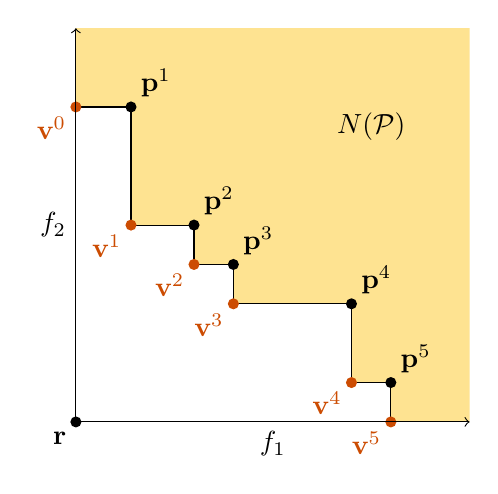
\begin{tikzpicture}
    
    % Shade the non-dominated area (above and right)
    \fill[fillcol] 
        (0,5) -- (0,4) -- (0.7,4) -- 
        (0.7,2.5) -- (1.5,2.5) -- 
        (1.5,2) -- (2,2) -- 
        (2,1.5) -- (3.5,1.5) -- 
        (3.5,0.5) -- (4,0.5) -- 
        (4,0) -- (5,0) -- (5,5) -- cycle;
    \node at (3.75,3.75) {\( N(\P) \)};


    % Draw lines from each point (downward and leftward)
    \draw (0.7,4) -- (0.7,2.5);  
    \draw (0.7,4) -- (0,4);      

    \draw (1.5,2.5) -- (1.5,2);  
    \draw (1.5,2.5) -- (0.7,2.5);

    \draw (2,2) -- (2,1.5);      
    \draw (2,2) -- (1.5,2);      

    \draw (3.5,1.5) -- (3.5,0.5);
    \draw (3.5,1.5) -- (2,1.5);  

    \draw (4,0.5) -- (4,0);      
    \draw (4,0.5) -- (3.5,0.5);  

    % Nondominated points
    \fill (0.7,4) circle (2pt) node[above right] {\( \textbf{p}^1 \)};
    \fill (1.5,2.5) circle (2pt) node[above right] {\( \textbf{p}^2 \)};
    \fill (2,2) circle (2pt) node[above right] {\( \textbf{p}^3 \)};
    \fill (3.5,1.5) circle (2pt) node[above right] {\( \textbf{p}^4 \)};
    \fill (4,0.5) circle (2pt) node[above right] {\( \textbf{p}^5 \)};

    % Intersection points v_0, ..., v_5
    \fill[nodecol] (0,4) circle (2pt) node[below left] {\( \textbf{v}^0 \)};
    \fill[nodecol] (0.7,2.5) circle (2pt) node[below left] {\( \textbf{v}^1 \)};
    \fill[nodecol] (1.5,2) circle (2pt) node[below left] {\( \textbf{v}^2 \)};
    \fill[nodecol] (2,1.5) circle (2pt) node[below left] {\( \textbf{v}^3 \)};
    \fill[nodecol] (3.5,0.5) circle (2pt) node[below left] {\( \textbf{v}^4 \)};
    \fill[nodecol] (4,0) circle (2pt) node[below left] {\( \textbf{v}^5 \)};


    % Draw axes
    \draw[->] (0,0) -- (5,0) node[midway, below] {\( f_1 \)};
    \draw[->] (0,0) -- (0,5) node[midway, left] {\( f_2 \)};
    
    % Draw a small dot at the origin
    \fill (0,0) circle (2pt) node[below left] {\( \textbf{r} \)};

\end{tikzpicture}

  \caption{Slika prikazuje množico točk $\P = \{\textbf{p}^1, \dots, \textbf{p}^5\}$, nedominirano območje $N(\P)$ ter vpete točke $\V(\P) = \{\textbf{v}^0, \dots, \textbf{v}^5\}$. Del množice $N(\P)$ je tudi rob, označen s črno črto.}
  \label{fig:nondominated_area}
\end{figure}

\begin{definicija}
Množici točk, ki šibko dominira neko točko $\textbf{z} \in \R^D$ rečemo \textit{stožec} in jo označimo s $C(\textbf{z})$. Primer dvodimenzionalnega stožca vidimo na sliki~\ref{fig:cone}.
\end{definicija}
\begin{figure}[htb]
  \centering
  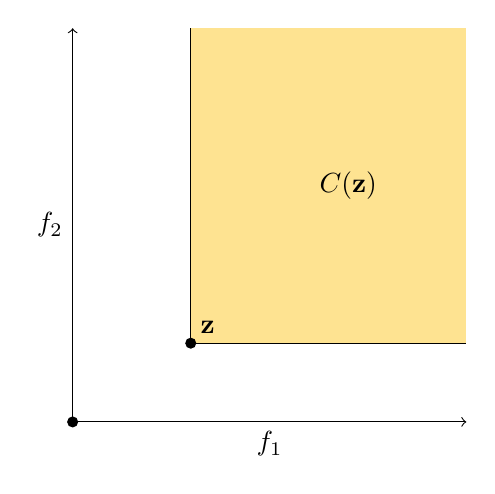
\begin{tikzpicture}
    
    % Shade the non-dominated area (above and right)
    \fill[fillcol] 
        (1.5,5) -- (5,5) -- (5,1) -- (1.5,1)  -- cycle;
    \node at (3.5,3) {\( C(\textbf{z}) \)};

    % Nondominated points
    \fill (1.5,1) circle (2pt) node[above right] {\( \textbf{z} \)};

    % Draw axes
    \draw[->] (0,0) -- (5,0) node[midway, below] {\( f_1 \)};
    \draw[->] (0,0) -- (0,5) node[midway, left] {\( f_2 \)};
    
    \draw (1.5,1) -- (1.5,5);
    \draw (1.5,1) -- (5,1);
    
    % Draw a small dot at the origin
    \fill (0,0) circle (2pt);

\end{tikzpicture}

  \caption{Na sliki sta prikazana točka $\textbf{z}$ in pripadajoči stožec $C(\textbf{z})$, označen z oranžnim območjem. Del stožca $C(z)$ je tudi rob, označen s črno črto.}
  \label{fig:cone}
\end{figure}

% \vspace{20cm}


\begin{definicija}
Točki $\textbf{v} \in N(\P)$ za katero velja
\[
\nexists \textbf{z} \in N(\P): \quad \textbf{v} \succ \textbf{z}
\]
rečemo \textit{vpeta točka}. Množico vseh vpetih točk $\textbf{v}$ za neko množico paroma nedominiranih točk $\P$ označimo z $\V(\P)$. Primer množice vpetih točk za množico dvodimenzionalnih točk $\P$ vidimo na sliki~\ref{fig:nondominated_area}.

Tekom dela računamo vpete točke za množice različnih dimenzij. Za to uporabimo različne algoritme, ki jih v nadaljevanju predstavimo. Verjamemo, da množice izračunanih vpetih točk natanko ustrezajo definiciji vpetih točk, vendar tega ne pokažemo. 
\end{definicija}



\input{vsebina/3_reševanje_problema}

\section{Testiranje implementacije}
\label{sec:analiza_pravilnosti}
V tem poglavju predstavimo postopek, s katerim testiramo pravilnost implementacije algoritma ARRNO. Kljub izpeljavi algoritma v prejšnjem poglavju, je testiranje vseeno pomembno. S tem pokažemo, da smo algoritem pravilno generalizirali v višje dimenzije, da deluje za posebne primere točk (na primer, kadar imajo točke iz $\P$ enako eno ali več koordinat), ter da se v implementacijo ni prikradla kakšna napaka. 

\subsection{Ideja testiranja}
Naj bo $\P$ množica paroma nedominiranih točk in $\textbf{q}$ točka poizvedbe. Za vsak $r \geq 0$ velja
\[
S(\textbf{q}, r) \cap N(\P) \neq \varnothing \iff d(\textbf{q}, N(\P)) \leq r,
\]
kjer je $S(\textbf{q}, r)$ sfera s središčem v $\textbf{q}$ in radijem $r$.

% Osnovna ideja testiranja algoritma je torej, da za veliko naključno izbranih kombinacij množic $\P$ in poizvedbenih točk $\textbf{q}$ z algoritmom izračunamo razdaljo $r_\text{A}$. Nato pa za nek majhen $\delta > 0$ preverimo, ali obstajata preseka $S(\textbf{q}, r_\text{A} - \delta) \cap N(\P)$ in $S(\textbf{q}, r_\text{A} + \delta) \cap N(\P)$. Primer treh točk poizvedbe in ustrezajočih sfer v dveh dimenzijah vidimo na sliki~\ref{fig:test_example}.

Osnovna ideja testiranja algoritma je torej, da za naključno izbrano kombinacijo množice $\P$ in poizvedbene točke $\textbf{q}$ z algoritmom ARRNO izračunamo razdaljo $r_\text{A}$. Nato pa za nek majhen $\delta > 0$ preverimo, ali obstajata preseka $S(\textbf{q}, r_\text{A} - \delta) \cap N(\P)$ in $S(\textbf{q}, r_\text{A} + \delta) \cap N(\P)$. Primer treh točk poizvedbe in ustrezajočih sfer v dveh dimenzijah vidimo na sliki~\ref{fig:test_example}. Če velja da je presek $S(\textbf{q}, r_\text{A} - \delta) \cap N(\P)$ prazen in $S(\textbf{q}, r_\text{A} + \delta) \cap N(\P)$ neprazen, potem vemo, da je napaka algoritma največ $\delta$. Če to velja za majhen $\delta$ pri veliko naključnih množicah $\P$ in poizvedbenih točkah $\textbf{q}$, smo lahko o pravilnosti algoritma precej prepričani. 
\begin{figure}[ht]
  \centering
  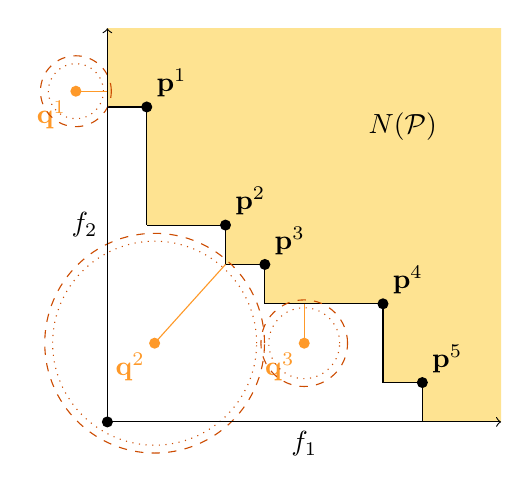
\begin{tikzpicture}
    
    % Shade the non-dominated area (above and right)
    \fill[fillcol] 
        (0,5) -- (0,4) -- (0.5,4) -- 
        (0.5,2.5) -- (1.5,2.5) -- 
        (1.5,2) -- (2,2) -- 
        (2,1.5) -- (3.5,1.5) -- 
        (3.5,0.5) -- (4,0.5) -- 
        (4,0) -- (5,0) -- (5,5) -- cycle;
    \node at (3.75,3.75) {\( N(\P) \)};


    % Draw lines from each point (downward and leftward)
    \draw (0.5,4) -- (0.5,2.5);  
    \draw (0.5,4) -- (0,4);      

    \draw (1.5,2.5) -- (1.5,2);  
    \draw (1.5,2.5) -- (0.5,2.5);

    \draw (2,2) -- (2,1.5);      
    \draw (2,2) -- (1.5,2);      

    \draw (3.5,1.5) -- (3.5,0.5);
    \draw (3.5,1.5) -- (2,1.5);  

    \draw (4,0.5) -- (4,0);      
    \draw (4,0.5) -- (3.5,0.5);  

    % Nondominated points
    \fill (0.5,4) circle (2pt) node[above right] {\( \textbf{p}^1 \)};
    \fill (1.5,2.5) circle (2pt) node[above right] {\( \textbf{p}^2 \)};
    \fill (2,2) circle (2pt) node[above right] {\( \textbf{p}^3 \)};
    \fill (3.5,1.5) circle (2pt) node[above right] {\( \textbf{p}^4 \)};
    \fill (4,0.5) circle (2pt) node[above right] {\( \textbf{p}^5 \)};

    % Additional points q1, q2, q3
    \fill[nodecol2] (-0.4,4.2) circle (2pt) node[below left] {\( \textbf{q}^1 \)};
    \draw[nodecol, dashed] (-0.4,4.2) ++(0:0.45) arc[start angle=0, end angle=360, radius=0.45];    
    \draw[nodecol, dotted] (-0.4,4.2) ++(0:0.35) arc[start angle=0, end angle=360, radius=0.35];    


    
    \fill[nodecol2] (0.6,1) circle (2pt) node[below left] {\( \textbf{q}^2 \)};
    \draw[nodecol, dashed] (0.6,1) ++(0:1.3453624 + 0.05) arc[start angle=0, end angle=360, radius=1.3453624 + 0.05];    
    \draw[nodecol, dotted] (0.6,1) ++(0:1.3453624 - 0.05) arc[start angle=0, end angle=360, radius=1.3453624 - 0.05];    

    
    \fill[nodecol2] (2.5,1) circle (2pt) node[below left] {\( \textbf{q}^3 \)};
    \draw[nodecol, dashed] (2.5,1) ++(0:0.55) arc[start angle=0, end angle=360, radius=0.55];    
    \draw[nodecol, dotted] (2.5,1) ++(0:0.45) arc[start angle=0, end angle=360, radius=0.45];    
    
    % Draw lines to the nearest boundary of the non-dominated region
    \draw[nodecol2] (-0.4,4.2) -- (0,4.2);  % q1 to shaded region (horizontally right)
    \draw[nodecol2] (0.6, 1) -- (1.5,2);  % q2 to v (diagonal)
    \draw[nodecol2] (2.5,1) -- (2.5,1.5);  % q3 to shaded region (vertically up)

    % Draw axes
    \draw[->] (0,0) -- (5,0) node[midway, below] {\( f_1 \)};
    \draw[->] (0,0) -- (0,5) node[midway, left] {\( f_2 \)};
    
    % Draw a small dot at the origin
    \fill (0,0) circle (2pt);

\end{tikzpicture}

  \caption{Tri točke poizvedbe $\textbf{q}^1$, $\textbf{q}^2$, $\textbf{q}^3$, skupaj z njihovimi razdaljami do nedominiranega območja ter ustrezajočimi sferami $S(\textbf{q}, r_\text{A} + \delta)$ s črtkano črto in $S(\textbf{q}, r_\text{A} - \delta)$ s točkasto črto.}
  \label{fig:test_example}
\end{figure}


\subsection{Diskretizacija sfere}
Da lahko računamo presek sfere z $N(\P)$, sfero diskretiziramo. Diskretizacija sfere $S(\textbf{q}, r)$ je množica točk, označimo jo z $\Sigma(\textbf{q}, r, \varepsilon)$, ki ležijo na $S(\textbf{q}, r)$ in za katere velja
\[
\forall \textbf{x} \in S(\textbf{q}, r): \quad \min_{\textbf{s} \in \Sigma(\textbf{q}, r, \varepsilon)} ||\textbf{x} - \textbf{s}|| \leq \varepsilon.
\]
Presek med diskretno sfero $\Sigma(\textbf{q}, r, \varepsilon)$ in $N(\P)$ lahko nato izračunamo enostavno
\[
\Sigma(\textbf{q}, r, \varepsilon) \cap N(\P) = \{ \textbf{s} \in \Sigma(\textbf{q}, r, \varepsilon) \mid \textbf{s} \succeq 0 \land \neg  (\P \ggcurly \textbf{s}) \}.
\]

Za lažjo notacijo v tem razdelku brez škode za splošnost predpostavljamo, da je sfera centrirana v koordinatnem izhodišču. Prav tako diskretiziramo le pozitivni del sfere, torej točke ki imajo vse koordinate nenegativne, kar označimo s $\Sigma^+(\textbf{0}, r, \varepsilon)$. V trditvi~\ref{trditev1} namreč pokažemo, da to zadošča za preverjanje preseka z nedominiranim območjem. 

\begin{trditev} \label{trditev1}
Vse komponente vektorja od poljubne točke $\textbf{q} \notin N(\P)$ do njej najbližje točke $\textbf{z} \in N(\P)$ so nenegativne.
\end{trditev}

\begin{dokaz}
Predpostavimo, da za neko množico $\P$ in točko $\textbf{q} = (q_1, \dots, q_D) \notin N(\P)$ obstaja točka $\textbf{z} = (z_1, \dots, z_D) \in N(\P)$, ki je najbližja točki $\textbf{q}$ izmed točk v $N(\P)$ ter da je $i$-ta komponenta vektorja $\textbf{w} = (z_1 - q_1, \dots, z_D - q_D)$ od $\textbf{q}$ do $\textbf{z}$ negativna. 

Potem definirajmo vektor $\textbf{w'} = (z_1 - q_1, \dots 0, \dots, z_D - q_D)$, ki je enak vektorju $\textbf{w}$, le da ima $i$-to komponento enako $0$, ter novo točko $\textbf{z'} = \textbf{q} + \textbf{w'}$.
Za točko $\textbf{z'} = (z_1, \dots, z_{i-1}, q_i, z_{i+1}, \dots, z_D)$ potem velja $\textbf{z'} \succ \textbf{z}$, saj je po predpostavki $q_i > z_i$, vse ostale komponente pa so enake. Ker je $\textbf{z} \in N(\P)$ in $\textbf{z'} \succ \textbf{z}$, je torej tudi $\textbf{z'} \in N(\P)$. Prav tako je očitno, da je $d(\textbf{q}, \textbf{z'}) = || \textbf{w'} || < || \textbf{w} || = d(\textbf{q}, \textbf{z})$, torej $\textbf{z}$ ni najbližja točka $\textbf{q}$ izmed točk v $N(\P)$, kar nas privede v protislovje. 
\end{dokaz}


Preprost način za konstrukcijo diskretne sfere $\Sigma^+(\textbf{0}, r, \varepsilon)$ je, da diskretiziramo površino sferi očrtane kocke $\Gamma^+(\textbf{0}, r, \varepsilon)$, nato pa točke projeciramo na sfero, kot je vidno na sliki~\ref{fig:constructing_sphere}.
\begin{figure}[ht]
    \begin{subfigure}{0.49\textwidth}
        \centering
        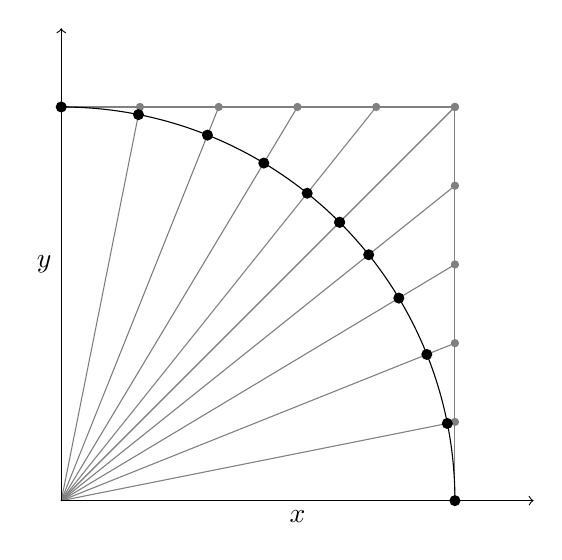
\begin{tikzpicture}

    \draw[gray] (5,0) -- (5,5);
    \draw[gray] (0,5) -- (5,5);

    \foreach \x in {0,1,2,3,4,5} {
        \draw[gray] (\x,5) -- (0,0);    
        \draw[gray] (5,\x) -- (0,0);    
        \fill[gray] (\x,5) circle (1.5pt);
        \fill[gray] (5,\x) circle (1.5pt);

        \pgfmathsetmacro{\r}{sqrt(\x*\x + 25)}
        \pgfmathsetmacro{\projx}{\x / \r * 5}
        \pgfmathsetmacro{\projy}{5 / \r * 5}

        \fill (\projx,\projy) circle (2pt);
        \fill (\projy,\projx) circle (2pt); 
    }

    \draw (5,0) arc[start angle=0, end angle=90, radius=5];    

    % Draw axes
    \draw[->] (0,0) -- (6,0) node[midway, below] {\( x \)};
    \draw[->] (0,0) -- (0,6) node[midway, left] {\( y \)};
\end{tikzpicture}

        \caption{Diskretizacija roba kocke in projekcija na sfero v dveh dimenzijah.}
        \label{fig:constructing_sphere_1}
    \end{subfigure}
    \hfill
    \begin{subfigure}{0.49\textwidth}
        \centering
        \tdplotsetmaincoords{70}{110}

\begin{tikzpicture}[scale=4,tdplot_main_coords]
\coordinate (O) at (0,0,0);
\draw[-stealth] (0,0,0) -- (1.2,0,0) node[anchor=north east]{$x$};
\draw[-stealth](0,0,0) -- (0,1.2,0) node[anchor=north west]{$y$};
\draw[-stealth] (0,0,0) -- (0,0,1.2) node[anchor=south]{$z$};

\draw[gray] (1,0,0) -- (1,1,0);
\draw[gray] (1,0,0) -- (1,0,1);
\draw[gray] (0,1,0) -- (1,1,0);
\draw[gray] (0,1,0) -- (0,1,1);
\draw[gray] (0,0,1) -- (1,0,1);
\draw[gray] (0,0,1) -- (0,1,1);
\draw[gray] (1,1,1) -- (0,1,1);
\draw[gray] (1,1,1) -- (1,0,1);
\draw[gray] (1,1,1) -- (1,1,0);

\foreach \x in {0,0.2,0.4,0.6,0.8,1} {
    \foreach \y in {0,0.2,0.4,0.6,0.8,1} {
        %\fill[gray] (\x,\y,1) circle (0.4pt);
        %\fill[gray] (\x,1,\y) circle (0.4pt);
        %\fill[gray] (1,\x,\y) circle (0.4pt);
        
        \pgfmathsetmacro{\r}{sqrt(\x*\x + \y*\y + 1)}
        \pgfmathsetmacro{\projx}{\x / \r}
        \pgfmathsetmacro{\projy}{\y / \r}
        \pgfmathsetmacro{\projz}{1 / \r}

        \draw[gray] (\projx,\projy,\projz) -- (\x,\y,1);
        \draw[gray] (\projx,\projz,\projy) -- (\x,1,\y);
        \draw[gray] (\projz,\projx,\projy) -- (1,\x,\y);

        \fill (\projx,\projy,\projz) circle (0.4pt);
        \fill (\projx,\projz,\projy) circle (0.4pt);
        \fill (\projz,\projx,\projy) circle (0.4pt);

        
    }
}






\tdplotsetthetaplanecoords{90}
% \tdplotdrawarc[tdplot_rotated_coords]{(0,0,0)}{0.5}{80}%
% {90}{anchor=west}{$d\phi_1$}
\draw[gray, dashed,tdplot_rotated_coords] (1,0,0) arc (0:90:1);

\draw[gray, dashed] (1,0,0) arc (0:90:1);

\tdplotsetthetaplanecoords{0}
\draw[gray, dashed,tdplot_rotated_coords] (1,0,0) arc (0:90:1);


\end{tikzpicture}
        \caption{Diskretizacija roba kocke in projekcija na sfero v treh dimenzijah.}
        \label{fig:constructing_sphere_2}
    \end{subfigure}
    \caption{Prikaz delovanja algoritma za diskretizacijo sfere v dveh in treh dimenzijah.}
    \label{fig:constructing_sphere}
\end{figure}

Pozitivni del hiperkocke v $D$ dimenzijah diskretiziramo tako, da združimo diskretizacijo vsake izmed $D$ pozitivnih stranic hiperkocke. Diskretizacija $i$-te stranice hiperkocke s stranico dolžine $r$ na $k+1$ točk je množica točk 
\[
\left\{0, \frac{1}{k}r, \frac{2}{k}r, \dots, \frac{k-1}{k}r, r\right\}^{i-1} \times \left\{ r \right\} \times \left\{0, \frac{1}{k}r, \frac{2}{k}r, \dots, \frac{k-1}{k}r, r\right\}^{D-i}.
\]
Torej je
\[
\Gamma^+(\textbf{0}, r, \varepsilon) = \bigcup_{i=1}^D \left\{0, \frac{1}{k}r, \frac{2}{k}r, \dots, \frac{k-1}{k}r, r\right\}^{i-1} \times \left\{ r \right\} \times \left\{0, \frac{1}{k}r, \frac{2}{k}r, \dots, \frac{k-1}{k}r, r\right\}^{D-i},
\]
iz česar pa enostavno dobimo diskretizacijo sfere $\Sigma^+(\textbf{q}, r, \varepsilon)$, tako da za vsako točko $\gamma \in \Gamma^+(\textbf{0}, r, \varepsilon)$ izračunamo njeno projekcijo $\sigma$ na sfero 
\[
\sigma = \frac{\gamma}{|| \gamma ||} r.
\]
Potrebno je le še določiti gostoto mreže, torej dolžino delitvenega intervala $\frac{r}{k}$. V dimenziji $D$ najbolj oddaljena točka $\textbf{x}$ od diskretne mreže leži ravno na sredini med točkami mreže, kot vidimo na sliki~\ref{fig:proof_h}, z maksimalno razdaljo enako 
\[
d_{\max} = \sqrt{(D-1)\frac{r^2}{(2k)^2}} = \frac{r}{2k}\sqrt{D-1}.
\]
Ker želimo da je $d_{\max} \leq \varepsilon$ mora veljati 
\[
\frac{r}{k} \leq \frac{2\varepsilon}{\sqrt{D-1}},
\]
kar velja za
\[
k = \left\lceil \frac{r \sqrt{D-1}}{2\varepsilon} \right\rceil.
\]
\begin{figure}[ht]
    \begin{subfigure}{0.32\textwidth}
        \centering
        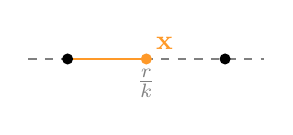
\begin{tikzpicture}
    \draw[gray, dashed] (-0.5, 1) -- (2.5, 1) node[midway, below] {$\frac{r}{k}$};    \draw[line width=0.3mm, nodecol2] (0, 1) -- (1, 1);      

    \fill (0,1) circle (2pt);
    \fill (2,1) circle (2pt);
    \fill[nodecol2] (1,1) circle (2pt) node[above right] {\( \textbf{x} \)};

\end{tikzpicture}

        %\caption{.}
        %\label{fig:proof_h2d}
    \end{subfigure}
    \hfill
    \begin{subfigure}{0.32\textwidth}
        \centering
        \begin{tikzpicture}

    \draw[gray, dashed] (-0.5, 0) -- (2.5, 0) node[midway, below] {$\frac{r}{k}$};    
    \draw[gray, dashed] (-0.5, 2) -- (2.5, 2);      
    \draw[gray, dashed] (0, -0.5) -- (0, 2.5);      
    \draw[gray, dashed] (2, -0.5) -- (2, 2.5);      

    % Draw a small dot at the origin
    \fill (0,0) circle (2pt);
    \fill (0,2) circle (2pt);
    \fill (2,0) circle (2pt);
    \fill (2,2) circle (2pt);

    \draw (0, 0) -- (1, 0);      
    \draw (1, 0) -- (1, 1);      
    
    \fill[nodecol2] (1,1) circle (2pt) node[above right] {\( \textbf{x} \)};
    \draw[line width=0.3mm, nodecol2] (1, 1) -- (0, 0);


\end{tikzpicture}

        %\caption{.}
        %\label{fig:proof_h3d}
    \end{subfigure}
    \hfill
    \begin{subfigure}{0.32\textwidth}
        \centering
        \tdplotsetmaincoords{70}{100}

\begin{tikzpicture}[scale=2,tdplot_main_coords]

\draw[gray, dashed] (1,-0.2,0) -- (1,1.2,0) node[midway, below] {$\frac{r}{k}$};
\draw[gray, dashed] (0,-0.2,0) -- (0,1.2,0);
\draw[gray, dashed] (1,0,-0.2) -- (1,0,1.2);
\draw[gray, dashed] (0,0,-0.2) -- (0,0,1.2);
\draw[gray, dashed] (-0.2,1,0) -- (1.2,1,0);
\draw[gray, dashed] (-0.2,0,0) -- (1.2,0,0);
\draw[gray, dashed] (0,1,-0.2) -- (0,1,1.2);
\draw[gray, dashed] (-0.2,0,1) -- (1.2,0,1);
\draw[gray, dashed] (0,-0.2,1) -- (0,1.2,1);
\draw[gray, dashed] (1.2,1,1) -- (-0.2,1,1);
\draw[gray, dashed] (1,1.2,1) -- (1,-0.2,1);
\draw[gray, dashed] (1,1,1.2) -- (1,1,-0.2);

\foreach \x in {0, 1} {
    \foreach \y in {0, 1} {
        \foreach \z in {0, 1} {
            \fill (\x,\y,\z) circle (1pt);
        }
    }
}

\draw (1,0,0) -- (1,0.5,0);
\draw (1,0.5,0) -- (0.5,0.5,0);
\draw (0.5,0.5,0.5) -- (0.5,0.5,0);

\draw[line width=0.3mm, nodecol2] (0.5,0.5,0.5) -- (1, 0, 0);
\fill[nodecol2] (0.5,0.5,0.5) circle (1pt) node[above right] {\( \textbf{x} \)};


\end{tikzpicture}

        %\caption{.}
        %\label{fig:proof_h4d}
    \end{subfigure}
    \caption{Primeri diskretizacij dela stranice dvodimenzionalne kocke na levi, tridimenzionalne kocke na sredini in štiridimenzionalne kocke na desni, skupaj s točko $\textbf{x}$, ki je od diskretizacije najbolj oddaljena.}
    \label{fig:proof_h}
\end{figure}

Za dobro izbiro $k$ torej velja, da je vsaka točka $\textbf{x}$ iz površine hiperkocke, največ za $\varepsilon$ oddaljena od diskretizacije. 
\begin{trditev}
\label{trditev:projekcija}
Za poljubni $D$-dimenzionalni točki $A$ in $B$ iz zunanjosti sfere in njuni projekciji na sfero $A'$ in $B'$ velja
\[
|| A' - B' || \leq || A - B ||. 
\]
\end{trditev}
\begin{dokaz}
Osredotočimo se lahko le na ravnino, ki gre skozi izhodišče sfere in točki $A$ in $B$, ki je prikazana na sliki~\ref{fig:sphere_contraction}. Naj bo $\theta$ kot med točkama $A$ in $B$ v tej ravnini. Po kosinusnem izreku je potem 
\[
||A' - B'||^2 = 2r^2 - 2r^2 \cos \theta,
\]
kjer je $r$ radij sfere in
\[
||A - B||^2 = (r + r_A)^2 + (r + r_B)^2 - 2(r + r_A) (r + r_B) \cos \theta,
\]
kjer sta $r + r_A$ in $r + r_B$ razdalji med izhodiščem sfere in točko $A$ oziroma $B$. Potem je
\[
||A - B||^2 - ||A' - B'||^2 = rr_A (2 - 2 \cos \theta) + rr_B (2 - 2 \cos \theta) + r_A^2 + r_B^2 - 2 r_A r_B \cos \theta
\]
Ker sta $r_A, r_B \geq 0$ očitno velja $rr_A (2 - 2 \cos \theta) \geq 0$ in $rr_B (2 - 2 \cos \theta) \geq 0$. Po kosinusnem izreku enako velja za $r_A^2 + r_B^2 - 2 r_A r_B \cos \theta$, saj je to ravno kvadrat dolžine nasprotne stranice trikotnika s stranicama $r_A$ in $r_B$ ter kotom $\theta$ med njima. Ker je torej $||A - B||^2 \geq ||A' - B'||^2$ je tudi $||A - B|| \geq ||A' - B'||$.
\begin{figure}[ht]
  \centering
  \begin{tikzpicture}

    \draw[gray] (0,0) -- (2.8284,2.8284);
    \draw[gray] (0,0) -- (2.058,3.43) node[midway, above] {\( r \)};
    
    \draw[gray] (2.8284,2.8284) -- (3.5, 3.5) node[midway, above, left] {\( r_B \)};
    \draw[gray] (2.058,3.43) -- (3,5) node[midway, above, left] {\( r_A \)};

    \draw (4,0) arc[start angle=0, end angle=90, radius=4];  
    \draw (2,2) arc[start angle=45, end angle=59.03, radius=2.828];  

    \draw[gray, dashed] (3,5) -- (3.5, 3.5);
    \draw[gray, dashed] (2.058,3.43) -- (2.8284,2.8284);

    \draw (1.55,2) node {\( \theta \)};


    \fill (3,5) circle (2pt) node[above right] {\( A \)};
    \fill (3.5, 3.5) circle (2pt) node[above right] {\( B \)};

    \fill (2.058,3.43) circle (2pt) node[above right] {\( A' \)};
    \fill (2.8284,2.8284) circle (2pt) node[right] {\( B' \)};


    % Draw axes
    \draw[->] (0,0) -- (6,0) node[midway, below] {\( x \)};
    \draw[->] (0,0) -- (0,6) node[midway, left] {\( y \)};
\end{tikzpicture}

  \caption{Slika prikazuje točki $A$ in $B$, njuni projekciji na sfero $A'$ in $B'$ ter razdalje $r$, $r_A$ in $r_B$.}
  \label{fig:sphere_contraction}
\end{figure}
\end{dokaz}

Po trditvi~\ref{trditev:projekcija} torej tudi za diskretizacijo sfere velja, da je vsaka točka $\textbf{x}$ iz površine sfere največ za $\varepsilon$ oddaljena od njene diskretizacije. 
\subsection{Gostota diskretizacije}
Za dani $\delta$ želimo izbrati tak $\varepsilon$, da je gostota diskretizacije dovolj velika in velja
\[
d(\textbf{q}, N(\P)) \leq r \implies \Sigma(\textbf{q}, r + \delta, \varepsilon) \cap N(\P) \neq \varnothing.
\]
Sicer bi se nam lahko zgodilo, da zaradi nesrečne izbire diskretizacije v preseku ne bi bilo nobene točke, kot je vidno na sliki~\ref{fig:determining-epsilon3}.
\begin{figure}[ht]
  \centering
  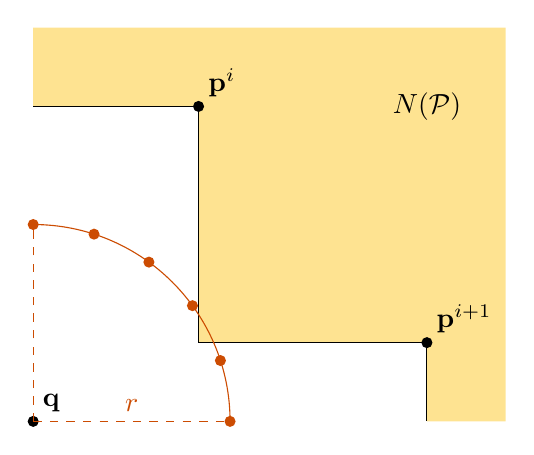
\begin{tikzpicture}
    
    % Shade the non-dominated area (above and right)
    \fill[fillcol] 
        (-2,4) -- (-2,3) -- (0.1,3) -- 
        (0.1, 0) -- (3,0) -- 
        (3, -1) -- (4,-1) -- (4,4) -- cycle;
    \node at (3,3) {\( N(\P) \)};


    % Draw lines from each point (downward and leftward)
    \draw (0.1,3) -- (-2,3);  
    \draw (0.1,3) -- (0.1,0);      

    \draw (3,0) -- (0.1,0);  
    \draw (3,0) -- (3, -1);  

    
    \fill (0.1,3) circle (2pt) node[above right] {\( \textbf{p}^i \)};
    \fill (3,0) circle (2pt) node[above right] {\( \textbf{p}^{i+1} \)};
    
     \fill (-2,-1) circle (2pt) node[above right] {\( \textbf{q} \)};
    \draw[nodecol, dashed] (-2,-1) -- (0.5,-1) node[midway, above] {$r$};  
    \draw[nodecol, dashed] (-2,-1) -- (-2,1.5);  
    \draw[nodecol] (0.5,-1) arc[start angle=0, end angle=90, radius=2.5];

    \foreach \x in {0, 18, 36, 54, 72, 90} {
        \fill[nodecol] ({-2 + 2.5* cos(\x)}, {-1 + 2.5* sin(\x)}) circle (2pt);
    }

    


\end{tikzpicture}

  \caption{Gostota diskretizacije sfere $S(\textbf{q}, r)$ je premajhna, da bi kakšna izmed točk diskretizacije $\Sigma(\textbf{q}, r, \varepsilon)$ padla v nedominirano območje $N(\P)$, kljub temu da je $d(\textbf{q}, N(\P)) < r$.}
  \label{fig:determining-epsilon3}
\end{figure}
Očitno je, da bomo za čim manjši $\delta$ potrebovali tem gostejšo diskretizacijo sfere. 
\begin{trditev}
\label{trditev:dokaz_pravilnosti}
Za izbiro $\varepsilon \leq \frac{\delta}{\sqrt{D}}$ velja
\[
d(\textbf{q}, N(\P)) \leq r \implies \Sigma(\textbf{q}, r + \delta, \varepsilon) \cap N(\P) \neq \varnothing.
\]
\end{trditev}
\begin{dokaz}
Oglejmo si sliko~\ref{fig:determining-epsilon1}, kjer vidimo primer točke $\textbf{q}$, ki je do najbližje točke $\textbf{v} \in N(\P)$ oddaljena za $r$. Prikazan je tudi pozitivni del sfere $S(\textbf{q}, r + \delta)$ s središčem v $\textbf{q}$ in radijem $r + \delta$ ter pozitivni del sfere $S(\textbf{v}, \delta)$ s središčem v $\textbf{v}$ in radijem $\delta$. Po trikotniški neenakosti sledi, da so vse točke na $S(\textbf{q}, r + \delta)$ od $\textbf{v}$ oddaljene več ali enako $\delta$. 
\begin{figure}[ht]
  \centering
  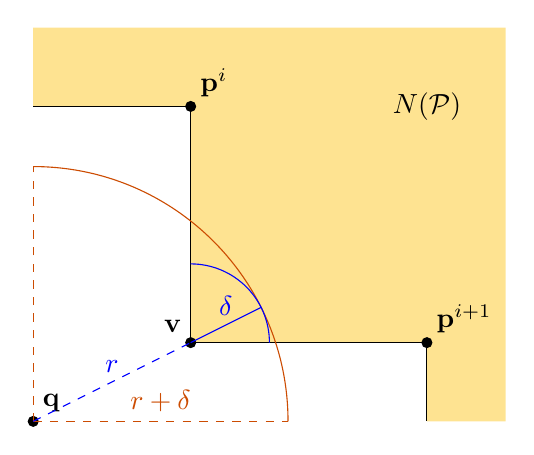
\begin{tikzpicture}
    
    % Shade the non-dominated area (above and right)
    \fill[fillcol] 
        (-2,4) -- (-2,3) -- (0,3) -- 
        (0, 0) -- (3,0) -- 
        (3, -1) -- (4,-1) -- (4,4) -- cycle;
    \node at (3,3) {\( N(\P) \)};


    % Draw lines from each point (downward and leftward)
    \draw (0,3) -- (-2,3);  
    \draw (0,3) -- (0,0);      

    \draw (3,0) -- (0,0);  
    \draw (3,0) -- (3, -1);  

    
    \fill (0,3) circle (2pt) node[above right] {\( \textbf{p}^i \)};
    \fill (3,0) circle (2pt) node[above right] {\( \textbf{p}^{i+1} \)};
    \fill (0,0) circle (2pt) node[above left] {\( \textbf{v}\)};
    
     \fill (-2,-1) circle (2pt) node[above right] {\( \textbf{q} \)};
    \draw[nodecol, dashed] (-2,-1) -- (1.23606798,-1) node[midway, above] {$r + \delta$};  
    \draw[nodecol, dashed] (-2,-1) -- (-2,2.23606798);  
    % \draw[nodecol, dashed] (0.23606798,-1) -- (1.23606798,-1) node[midway, above] {$\delta$};
    \draw[nodecol] (1.23606798,-1) arc[start angle=0, end angle=90, radius=3.23606798];    
    % \draw[nodecol, dashed] (0.23606798,-1) arc[start angle=0, end angle=90, radius=2.23606798];    
    \draw[blue, dashed] (-2,-1) -- (0,0) node[midway, above] {$r$};
    \draw[blue] (0.8944272,0.4472136) -- (0,0) node[midway, above] {$\delta$};
    \draw[blue] (1, 0) arc[start angle=0, end angle=90, radius=1];    
    % \fill[blue] (0.70710678,0.70710678) circle (1pt) node[left] {$\overline{\textbf{s}}$};
    
    
    % \draw[gray, dashed] (1,1) -- (0,0);
    % \fill[gray] (0.73295,0.73295) circle (1pt) node[right] {\( \textbf{s} \)};

    % \draw[blue, dashed] (0.707106781,0.707106781) circle (0.707106781); 



\end{tikzpicture}

  \caption{Slika prikazuje primer točke $\textbf{q}$ ter njej najbližjo točko iz $N(P)$, točko $\textbf{v}$. Z oranžno barvo je prikazana testna sfera  $S(\textbf{q}, r + \delta)$, z modro barvo pa $S(\textbf{v}, \delta)$.}
  \label{fig:determining-epsilon1}
\end{figure}

Skozi $\textbf{v}$ nato potegnemo premico $l$ pod kotom $45^\circ$ na vse koordinatne osi, ki seka $S(\textbf{v}, \delta)$ v točki $\textbf{s}$, kot vidimo na sliki~\ref{fig:determining-epsilon2}. Po podobnem razmisleku, kot na sliki~\ref{fig:proof_h} je jasno, da je vektor od $\textbf{v}$ do $\textbf{s}$ enak $(\frac{\delta}{\sqrt{D}}, \dots, \frac{\delta}{\sqrt{D}})$. Torej krogla $B(\textbf{s}, \frac{\delta}{\sqrt{D}})$ v celoti leži znotraj $N(\P)$. Naj bo $I = S(\textbf{v}, \delta) \cap B(\textbf{s}, \frac{\delta}{\sqrt{D}})$ del sfere $S(\textbf{v}, \delta)$, ki leži znotraj krogle $B(\textbf{s}, \frac{\delta}{\sqrt{D}})$. Množica $I \subset N(\P)$ vsebuje vse točke iz $S(\textbf{v}, \delta)$, ki so od $\textbf{s}$ oddaljene manj kot $\frac{\delta}{\sqrt{D}}$. Torej pri vsaki diskretizaciji $S(\textbf{v}, \delta)$ z $\varepsilon \leq \frac{\delta}{\sqrt{D}}$ obstaja točka diskretizacije, ki leži v $I$ torej leži tudi v $N(\P)$.
\begin{figure}[ht]
  \centering
  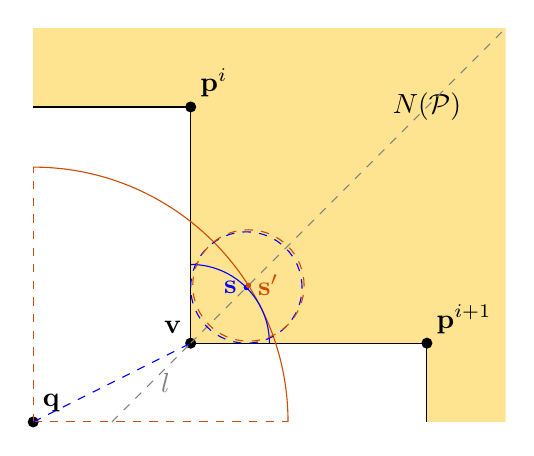
\begin{tikzpicture}
    
    % Shade the non-dominated area (above and right)
    \fill[fillcol] 
        (-2,4) -- (-2,3) -- (0,3) -- 
        (0, 0) -- (3,0) -- 
        (3, -1) -- (4,-1) -- (4,4) -- cycle;
    \node at (3,3) {\( N(\P) \)};


    % Draw lines from each point (downward and leftward)
    \draw (0,3) -- (-2,3);  
    \draw (0,3) -- (0,0);      

    \draw (3,0) -- (0,0);  
    \draw (3,0) -- (3, -1);  

    
    \fill (0,3) circle (2pt) node[above right] {\( \textbf{p}^i \)};
    \fill (3,0) circle (2pt) node[above right] {\( \textbf{p}^{i+1} \)};
    \fill (0,0) circle (2pt) node[above left] {\( \textbf{v}\)};
    \fill (-2,-1) circle (2pt) node[above right] {\( \textbf{q} \)};
    
    \draw[nodecol, dashed] (-2,-1) -- (1.23606798,-1);  
    \draw[nodecol, dashed] (-2,-1) -- (-2,2.23606798);  
    % \draw[nodecol, dashed] (0.23606798,-1) -- (1.23606798,-1) node[midway, above] {$\delta$};
    \draw[nodecol] (1.23606798,-1) arc[start angle=0, end angle=90, radius=3.23606798];    
    \draw[blue, dashed] (-2,-1) -- (0,0);
    % \draw[blue] (0.8944272,0.4472136) -- (0,0) node[midway, above] {$\delta$};
    \draw[blue] (1, 0) arc[start angle=0, end angle=90, radius=1];    
    \fill[blue] (0.70710678,0.70710678) circle (1pt) node[left] {$\textbf{s}$};
    
    
    \draw[gray, dashed] (0,0) -- (4,4);
    \draw[gray, dashed] (-1,-1) -- (0,0) node[midway, right] {\( l \)};
    \draw[blue, dashed] (0.707106781,0.707106781) circle (0.707106781); 

    \fill[nodecol] (0.73295,0.73295) circle (1pt) node[right] {\( \textbf{s}' \)};
    \draw[nodecol, dashed]  (0.73295,0.73295) circle (0.707106781);    



\end{tikzpicture}

  \caption{S sivo črto je prikazana premica $l$, ki gre skozi točko $\textbf{v}$, ter seka modro oziroma oranžno sfero v točkah $\textbf{s}$ ter $\textbf{s}'$. Okrog točk $\textbf{s}$ in $\textbf{s}'$ sta prikazani sferi z radijem $\frac{\delta}{\sqrt{D}}$.}
  \label{fig:determining-epsilon2}
\end{figure}

Podobno lahko definiramo točko $\textbf{s}'$, ki je na presečišču premice $l$ in sfere $S(\textbf{q}, r + \delta)$. Ker je del sfere $S(\textbf{q}, r + \delta)$, ki je znotraj $N(\P)$, kvečjemu dlje od $\textbf{v}$ kot $S(\textbf{v}, \delta)$, bo po enakem razmisleku veljalo, da je diskretizacija z $\varepsilon \leq \frac{\delta}{\sqrt{D}}$ dovolj natančna tudi za $S(\textbf{q}, r + \delta)$.

\end{dokaz}


\subsection{Testiranje}
Naj bo $r_{\text{A}}$ z algoritmom izračunana razdalja med nedominiranim območjem dane množice $\P$ ter poizvedbene točke $\textbf{q}$. Za nek majhen $\delta$ bi radi pokazali da velja $d(\textbf{q}, N(\P)) - \delta \leq r_\text{A} \leq d(\textbf{q}, N(\P)) + \delta$. 

\subsubsection{Spodnja meja}
Izberemo $\varepsilon = \frac{\delta}{\sqrt{D}}$ in preverimo presek $\Sigma(\textbf{q}, r_{\text{A}} + \delta, \varepsilon) \cap N(\P)$. Če presek vsebuje kako točko, vemo da velja $d(\textbf{q}, N(\P)) \leq r_\text{A} + \delta$ oziroma $d(\textbf{q}, N(\P)) - \delta \leq r_\text{A}$. Sicer pa po trditvi~\ref{trditev:dokaz_pravilnosti} vemo, da je $d(\textbf{q}, N(\P)) > r_\text{A}$ torej algoritem ne deluje pravilno. 

\subsubsection{Zgornja meja}
Iz trditve~\ref{trditev:dokaz_pravilnosti} po kontrapoziciji velja
\[
\Sigma(\textbf{q}, r, \varepsilon) \cap N(\P) = \varnothing \implies d(\textbf{q}, N(\P)) > r - \delta,
\]
pri izbiri $\varepsilon = \frac{\delta}{\sqrt{D}}$. Presek $\Sigma(\textbf{q}, r_\text{A}, \varepsilon) \cap N(\P)$ ob pravilnem delovanju algoritma ni nujno prazen, zato preverimo presek $\Sigma(\textbf{q}, r_\text{A} - \mu, \varepsilon') \cap N(\P)$, kjer je $\mu = \frac{\delta}{10^6}$, $\varepsilon' = \frac{\delta'}{\sqrt{D}}$ in $\delta' = \delta - \mu$. Če presek ni prazen, vemo da algoritem deluje narobe, sicer pa napako omejimo na
\[
r_\text{A} - \mu - (\delta - \mu) < d(\textbf{q}, N(\P)),
\]
iz česar sledi
\[
r_\text{A} \leq d(\textbf{q}, N(\P)) + \delta.
\]

\subsubsection{Rezultati testiranja}
Algoritem testiramo za dimenzije 3, 4, 5 in 6. Pri vsaki dimenziji ponovimo 100 poskusov z različnimi množicami $\P$ in točkami $\textbf{q}$. Da dobimo množico $\P$, naključno izberemo 100 točk iz $[0, 1]^D$ in odstranimo dominirane. Da dobimo točko $\textbf{q}$, prav tako naključno izbiramo točke iz $[0, 1]^D$, dokler $\P$ točke ne dominira. Nato z algoritmom ARRNO izračunamo razdaljo $r_\text{A}$ med točko $\textbf{q}$ ter nedominiranim območjem množice $\P$. Rezultate testiramo za čim manjše vrednosti $\delta$, kolikor nam omogočajo zmogljivosti strojne opreme. Ker za preverjanje preseka $\Sigma(\textbf{q}, r, \varepsilon) \cap N(\P)$ preverimo vsako kombinacijo točk iz $\Sigma(\textbf{q}, r, \varepsilon)$ in iz $\P$, za to potrebujemo $O(|\Sigma(\textbf{q}, r, \varepsilon)| \cdot |\P|)$ primerjav. Vrednost $\delta$ izberemo v odvisnosti od $r_\text{A}$, da je število točk diskretizacije vedno enako. Prav tako za višje dimenzije izberemo večji $\delta$, saj se število točk diskretizacije z dimenzijo veča. Tabela~\ref{tab:vrednosti_delta} prikazuje vrednosti $\delta$ in velikost diskretizacije sfere za različne dimenzije.
\begin{table}[htb]
    \centering
    \begin{tabular}{c r r}
        dimenzija & vrednost $\delta$ & št.~točk diskretizacije  \\
        \hline
        3 & $0.001 \cdot r_\text{A}$ & $\sim 4.5 \cdot 10^6$ \\
        4 & $0.01 \cdot r_\text{A}$ & $\sim 21.6 \cdot 10^6$ \\
        5 & $0.05 \cdot r_\text{A}$ & $\sim 25.5 \cdot 10^6$ \\
        6 & $0.2 \cdot r_\text{A}$ & $\sim 9.9 \cdot 10^6$ \\
    \end{tabular}
    \caption{Tabela prikazuje izbrane vrednosti za $\delta$ pri različnih dimenzijah, povprečno število točk diskretizacije sfere z izbranim $\delta$ ter povprečno število vpetih točk.}
    \label{tab:vrednosti_delta}
\end{table}

Da testiramo tudi primer, ko imata dve ali več točk kakšno izmed koordinat enako, vse poskuse ponovimo, le da tokrat točke za množico $\P$ izbiramo naključno iz $\{0.1, 0.2, \dots, 0.9, 1 \}^D$. Tako je verjetnost, da imata dve točki neko koordinato enako precej večja. Poskuse prav tako ponovimo še za primer, ko točka $\textbf{q} \notin [0, 1]^D$. Tokrat jo naključno izberemo iz množice $[-1, 1]^D \setminus [0, 1]^D$. 

Skupaj torej naključno ustvarimo $800$ testnih problemov, na katerih preverimo delovanje. Testiranje na namiznem računalniku s 16 GB pomnilnika
in frekvenco procesorja 3,60 GHz traja nekaj dni. V vseh primerih algoritem ARRNO deluje pravilno, kar kaže na to, da je zasnova in implementacija pravilna.  



\section{Računska zahtevnost}
\label{sec:racunska_zahtevnost}
V tem poglavju podrobno analiziramo računsko zahtevnost algoritma v odvisnosti od velikosti množice nedominiranih točk $n = |\P|$ ter dimenzije problema $D$. Za lažjo analizo predpostavljamo, da je dimenzija $D$ konstanta, torej da lahko namesto $O(D)$ pišemo $O(1)$\footnote{Seveda pa dimenzije $D$ ne zanemarimo, ko ta nastopa v eksponentu.}. Predpostavka je smiselna, saj je računanje enostavnejših indikatorjev pri visokih dimenzijah zelo zamudno, tako da se v praksi le redko srečamo z več kot nekaj kriteriji. 

Najprej teoretično analiziramo časovno ter prostorsko zahtevnost, nato pa hitrost algoritma tudi testiramo za probleme dimenzij od 3 do 6, na množicah točk različnih velikost in oblik. Na koncu analiziramo še scenarij, kjer je algoritmu za množico paroma nedominiranih točk $\P$ danih več točk poizvedbe $\Q = \{\textbf{q}^1, \dots, \textbf{q}^m \}$ naenkrat. 

\subsection{Teoretična analiza časovne zahtevnosti}
\begin{izrek}
Algoritem ARRNO za računanje razdalje med nedominiranim območjem $N(\P)$ in točko poizvedbe $\textbf{q}$, ima časovno zahtevnost $O(n \log n)$ za $D=3$ in $O(n^{D-1})$ za $D \geq 4$, kjer je $n = |\P|$ in $D$ dimenzija prostora.
\end{izrek}
Časovna zahtevnost algoritma ARRNO je sestavljena iz časovne zahtevnosti računanja množice vpetih točk $\V$ ter časovne zahtevnosti iskanja razdalje do najbližjega stožca, ki ga razpenjajo vpete točke. Naj bo število vpetih točk enako $v$. Potem očitno poiščemo najbližji stožec v $O(v)$. Ker pa smo pri konstrukciji vpetih točk gotovo konstruirali vsako izmed njih, je časovna zahtevnost iskanja vpetih točk vsaj $O(v)$. Torej zadošča izračunati časovno zahtevnost algoritma \Call{Vpete točke}{$\P$}. Vseeno pa najprej pokažimo, kolikšno je maksimalno število vpetih točk $\V$, glede na dimenzijo problema. 

\begin{trditev}
\label{sec:st_vpetih_tock}
Za dimenzijo $D=2, 3$ je število vpetih točk $O(n)$, kjer je $n = |\P|$. Za $D=4$ je število vpetih točk $O(n^2)$ in obstajajo take množice točk $\P$, za katere je število vpetih točk $\Omega(n^2)$. Za $D > 4$ je število vpetih točk $O(n^{D-2})$.
\end{trditev}

\begin{dokaz}
V algoritmu \Call{Vpete točke 3D}{$\P$}, za računanje vpetih točk v treh dimenzijah, na vsakem koraku zanke (algoritem \ref{alg:vpete_tocke_3d}, vrstice 6--16) v stanje $\sv$ dodamo največ dve točki. Skupaj s točko $(0, 0)$, ki je v množici $\sv$ od začetka, torej v $\sv$ dodamo največ $2n + 1$ točk. Ker vpete točke računamo tako, da jih postopoma odstranjujemo iz $\sv$, bo tudi vpetih točk največ $2n + 1$. 
    
Kadar rešujemo problem v štirih dimenzijah  (algoritem \ref{alg:vpete_tocke}, vrstica 14), $n$-krat dodamo vpete točke tridimenzionalnega podproblema. Torej je vpetih točk v štirih dimenzijah največ
\[
1 + \sum_{i=1}^n 2i + 1 = (n + 1) + 2 \sum_{i=1}^n i = (n + 1) + n(n + 1) = (n + 1)^2 = O(n^2).
\] 
Da je kvadratično število vpetih točk v štirih dimenzijah res tesna meja, pokažemo na primeru. Sestavimo tak primer, kjer pri dodajanju prve polovice točk vsakič dobimo konstantno število vpetih točk, pri dodajanju druge polovice točk, pa vsakič linearno število novih vpetih točk. Tak primer je na primer množica točk
\[
\left \{(i + 1, \frac{n}{2} - i, n - i, n - i) \mid  i = 0, 1, \dots \frac{n}{2} - 1 \right \},
\]
za prvo polovico točk, ter 
\[
\left \{(n - i, n - i, i + 1, \frac{n}{2} - i) \mid  i = 0, 1, \dots \frac{n}{2} - 1 \right \},
\]
za drugo polovico točk. Na sliki~\ref{fig:example4d} vidimo vizualizacijo tridimenzionalnega stanja $\sp$ za primer $n = 6$ po dodajanju prvih treh, štirih, petih in šestih točk. 

\begin{figure}[ht]
    \centering
    \begin{subfigure}{0.495\textwidth}
        \centering
        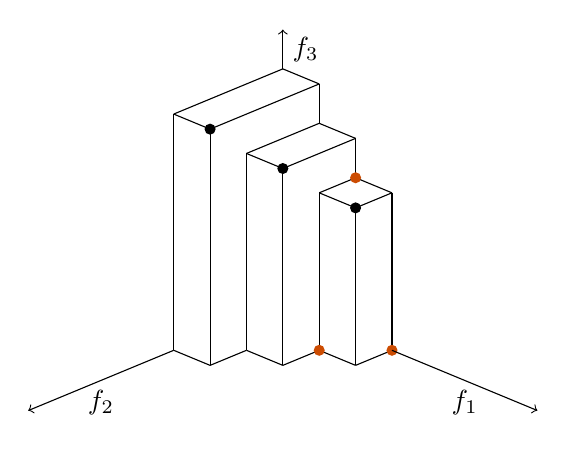
\begin{tikzpicture}
    % lines:
    \draw (-0.9239,2.2346) -- (-1.3858,2.426);
    \draw (-1.3858,2.426) -- (0.0,3.0);
    \draw (-1.3858,2.426) -- (-1.3858,-0.574);
    \draw (-0.9239,2.2346) -- (0.4619,2.8087);
    \draw (0.4619,2.8087) -- (0.0,3.0);
    \draw (0.4619,2.8087) -- (0.4619,2.3087);
    \draw (-0.9239,2.2346) -- (-0.9239,-0.7654);
    \draw (-0.9239,-0.7654) -- (-1.3858,-0.574);
    \draw (-0.9239,-0.7654) -- (-0.4619,-0.574);
    \draw (0.0,1.7346) -- (-0.4619,1.926);
    \draw (-0.4619,1.926) -- (0.4619,2.3087);
    \draw (-0.4619,1.926) -- (-0.4619,-0.574);
    \draw (0.0,1.7346) -- (0.9239,2.1173);
    \draw (0.9239,2.1173) -- (0.4619,2.3087);
    \draw (0.9239,2.1173) -- (0.9239,1.6173);
    \draw (0.0,1.7346) -- (0.0,-0.7654);
    \draw (0.0,-0.7654) -- (-0.4619,-0.574);
    \draw (0.0,-0.7654) -- (0.4619,-0.574);
    \draw (0.9239,1.2346) -- (0.4619,1.426);
    \draw (0.4619,1.426) -- (0.9239,1.6173);
    \draw (0.4619,1.426) -- (0.4619,-0.574);
    \draw (0.9239,1.2346) -- (1.3858,1.426);
    \draw (1.3858,1.426) -- (0.9239,1.6173);
    \draw (1.3858,1.426) -- (1.3858,-0.574);
    \draw (0.9239,1.2346) -- (0.9239,-0.7654);
    \draw (0.9239,-0.7654) -- (0.4619,-0.574);
    \draw (0.9239,-0.7654) -- (1.3858,-0.574);
    % points:
    \fill[black] (-0.9238795325112866,2.2346331352698203) circle (2pt) ;
    \fill[black] (0.0,1.7346331352698203) circle (2pt) ;
    \fill[black] (0.9238795325112866,1.2346331352698203) circle (2pt) ;
    % kink points:
    \fill[nodecol] (0.9238795325112867,1.6173165676349102) circle (2pt) ;
    \fill[nodecol] (0.46193976625564337,-0.5740251485476346) circle (2pt) ;
    \fill[nodecol] (1.38581929876693,-0.5740251485476346) circle (2pt) ;
    % axes:
    \draw[->] (1.3858,-0.574) -- (3.2336,-1.3394) node[midway, below] {\( f_1 \)};
    \draw[->] (-1.3858,-0.574) -- (-3.2336,-1.3394) node[midway, below] {\( f_2 \)};
    \draw[->] (0.0,3.0) -- (0.0,3.5) node[midway, right] {\( f_3 \)};
\end{tikzpicture}
        \caption{Stanje po dodajanju tretje točke.}
        \label{example4d_1}
    \end{subfigure}
    \hfill
    \begin{subfigure}{0.495\textwidth}
        \centering
        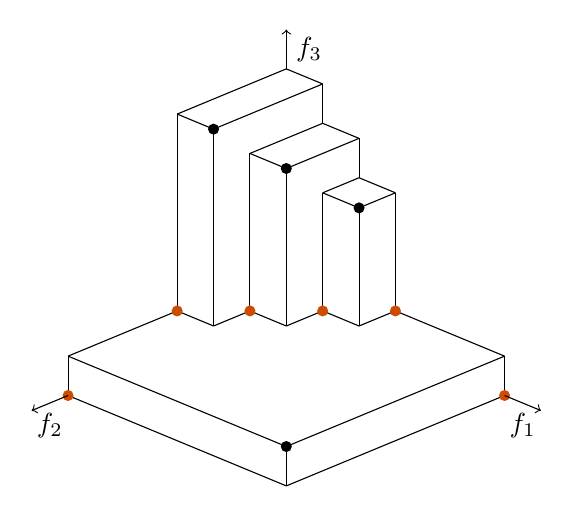
\begin{tikzpicture}
    % lines:
    \draw (-0.9239,2.2346) -- (-1.3858,2.426);
    \draw (-1.3858,2.426) -- (0.0,3.0);
    \draw (-1.3858,2.426) -- (-1.3858,-0.074);
    \draw (-0.9239,2.2346) -- (0.4619,2.8087);
    \draw (0.4619,2.8087) -- (0.0,3.0);
    \draw (0.4619,2.8087) -- (0.4619,2.3087);
    \draw (-0.9239,2.2346) -- (-0.9239,-0.2654);
    \draw (-0.9239,-0.2654) -- (-1.3858,-0.074);
    \draw (-0.9239,-0.2654) -- (-0.4619,-0.074);
    \draw (0.0,1.7346) -- (-0.4619,1.926);
    \draw (-0.4619,1.926) -- (0.4619,2.3087);
    \draw (-0.4619,1.926) -- (-0.4619,-0.074);
    \draw (0.0,1.7346) -- (0.9239,2.1173);
    \draw (0.9239,2.1173) -- (0.4619,2.3087);
    \draw (0.9239,2.1173) -- (0.9239,1.6173);
    \draw (0.0,1.7346) -- (0.0,-0.2654);
    \draw (0.0,-0.2654) -- (-0.4619,-0.074);
    \draw (0.0,-0.2654) -- (0.4619,-0.074);
    \draw (0.9239,1.2346) -- (0.4619,1.426);
    \draw (0.4619,1.426) -- (0.9239,1.6173);
    \draw (0.4619,1.426) -- (0.4619,-0.074);
    \draw (0.9239,1.2346) -- (1.3858,1.426);
    \draw (1.3858,1.426) -- (0.9239,1.6173);
    \draw (1.3858,1.426) -- (1.3858,-0.074);
    \draw (0.9239,1.2346) -- (0.9239,-0.2654);
    \draw (0.9239,-0.2654) -- (0.4619,-0.074);
    \draw (0.9239,-0.2654) -- (1.3858,-0.074);
    \draw (0.0,-1.7961) -- (-2.7716,-0.6481);
    \draw (-2.7716,-0.6481) -- (-1.3858,-0.074);
    \draw (-2.7716,-0.6481) -- (-2.7716,-1.1481);
    \draw (0.0,-1.7961) -- (2.7716,-0.6481);
    \draw (2.7716,-0.6481) -- (1.3858,-0.074);
    \draw (2.7716,-0.6481) -- (2.7716,-1.1481);
    \draw (0.0,-1.7961) -- (0.0,-2.2961);
    \draw (0.0,-2.2961) -- (-2.7716,-1.1481);
    \draw (0.0,-2.2961) -- (2.7716,-1.1481);
    % points:
    \fill[black] (-0.9238795325112866,2.2346331352698203) circle (2pt) ;
    \fill[black] (0.0,1.7346331352698203) circle (2pt) ;
    \fill[black] (0.9238795325112866,1.2346331352698203) circle (2pt) ;
    \fill[black] (0.0,-1.7961005941905386) circle (2pt) ;
    % kink points:
    \fill[nodecol] (-1.38581929876693,-0.07402514854763464) circle (2pt) ;
    \fill[nodecol] (-0.46193976625564337,-0.07402514854763464) circle (2pt) ;
    \fill[nodecol] (0.46193976625564337,-0.07402514854763464) circle (2pt) ;
    \fill[nodecol] (1.38581929876693,-0.07402514854763464) circle (2pt) ;
    \fill[nodecol] (-2.77163859753386,-1.1480502970952693) circle (2pt) ;
    \fill[nodecol] (2.77163859753386,-1.1480502970952693) circle (2pt) ;
    % axes:
    \draw[->] (2.7716,-1.1481) -- (3.2336,-1.3394) node[midway, below] {\( f_1 \)};
    \draw[->] (-2.7716,-1.1481) -- (-3.2336,-1.3394) node[midway, below] {\( f_2 \)};
    \draw[->] (0.0,3.0) -- (0.0,3.5) node[midway, right] {\( f_3 \)};
\end{tikzpicture}
        \caption{Stanje po dodajanju četrte točke.}
        \label{example4d_2}
    \end{subfigure}

    \vspace{0.5cm}

    \begin{subfigure}{0.495\textwidth}
        \centering
        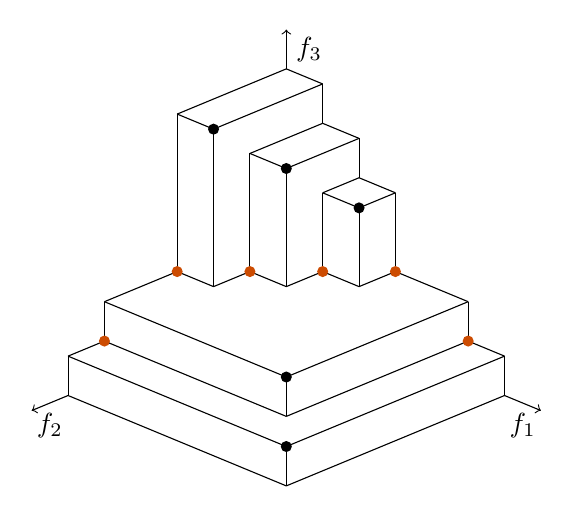
\begin{tikzpicture}
    % lines:
    \draw (-0.9239,2.2346) -- (-1.3858,2.426);
    \draw (-1.3858,2.426) -- (0.0,3.0);
    \draw (-1.3858,2.426) -- (-1.3858,0.426);
    \draw (-0.9239,2.2346) -- (0.4619,2.8087);
    \draw (0.4619,2.8087) -- (0.0,3.0);
    \draw (0.4619,2.8087) -- (0.4619,2.3087);
    \draw (-0.9239,2.2346) -- (-0.9239,0.2346);
    \draw (-0.9239,0.2346) -- (-1.3858,0.426);
    \draw (-0.9239,0.2346) -- (-0.4619,0.426);
    \draw (0.0,1.7346) -- (-0.4619,1.926);
    \draw (-0.4619,1.926) -- (0.4619,2.3087);
    \draw (-0.4619,1.926) -- (-0.4619,0.426);
    \draw (0.0,1.7346) -- (0.9239,2.1173);
    \draw (0.9239,2.1173) -- (0.4619,2.3087);
    \draw (0.9239,2.1173) -- (0.9239,1.6173);
    \draw (0.0,1.7346) -- (0.0,0.2346);
    \draw (0.0,0.2346) -- (-0.4619,0.426);
    \draw (0.0,0.2346) -- (0.4619,0.426);
    \draw (0.9239,1.2346) -- (0.4619,1.426);
    \draw (0.4619,1.426) -- (0.9239,1.6173);
    \draw (0.4619,1.426) -- (0.4619,0.426);
    \draw (0.9239,1.2346) -- (1.3858,1.426);
    \draw (1.3858,1.426) -- (0.9239,1.6173);
    \draw (1.3858,1.426) -- (1.3858,0.426);
    \draw (0.9239,1.2346) -- (0.9239,0.2346);
    \draw (0.9239,0.2346) -- (0.4619,0.426);
    \draw (0.9239,0.2346) -- (1.3858,0.426);
    \draw (0.0,-1.7961) -- (-2.7716,-0.6481);
    \draw (-2.7716,-0.6481) -- (-2.3097,-0.4567);
    \draw (-2.7716,-0.6481) -- (-2.7716,-1.1481);
    \draw (0.0,-1.7961) -- (2.7716,-0.6481);
    \draw (2.7716,-0.6481) -- (2.3097,-0.4567);
    \draw (2.7716,-0.6481) -- (2.7716,-1.1481);
    \draw (0.0,-1.7961) -- (0.0,-2.2961);
    \draw (0.0,-2.2961) -- (-2.7716,-1.1481);
    \draw (0.0,-2.2961) -- (2.7716,-1.1481);
    \draw (0.0,-0.9134) -- (-2.3097,0.0433);
    \draw (-2.3097,0.0433) -- (-1.3858,0.426);
    \draw (-2.3097,0.0433) -- (-2.3097,-0.4567);
    \draw (0.0,-0.9134) -- (2.3097,0.0433);
    \draw (2.3097,0.0433) -- (1.3858,0.426);
    \draw (2.3097,0.0433) -- (2.3097,-0.4567);
    \draw (0.0,-0.9134) -- (0.0,-1.4134);
    \draw (0.0,-1.4134) -- (-2.3097,-0.4567);
    \draw (0.0,-1.4134) -- (2.3097,-0.4567);
    % points:
    \fill[black] (-0.9238795325112866,2.2346331352698203) circle (2pt) ;
    \fill[black] (0.0,1.7346331352698203) circle (2pt) ;
    \fill[black] (0.9238795325112866,1.2346331352698203) circle (2pt) ;
    \fill[black] (0.0,-1.7961005941905386) circle (2pt) ;
    \fill[black] (0.0,-0.913417161825449) circle (2pt) ;
    % kink points:
    \fill[nodecol] (-1.38581929876693,0.42597485145236536) circle (2pt) ;
    \fill[nodecol] (-0.46193976625564337,0.42597485145236536) circle (2pt) ;
    \fill[nodecol] (0.46193976625564337,0.42597485145236536) circle (2pt) ;
    \fill[nodecol] (1.38581929876693,0.42597485145236536) circle (2pt) ;
    \fill[nodecol] (-2.309698831278217,-0.4567085809127245) circle (2pt) ;
    \fill[nodecol] (2.309698831278217,-0.4567085809127245) circle (2pt) ;
    % axes:
    \draw[->] (2.7716,-1.1481) -- (3.2336,-1.3394) node[midway, below] {\( f_1 \)};
    \draw[->] (-2.7716,-1.1481) -- (-3.2336,-1.3394) node[midway, below] {\( f_2 \)};
    \draw[->] (0.0,3.0) -- (0.0,3.5) node[midway, right] {\( f_3 \)};
\end{tikzpicture}
        \caption{Stanje po dodajanju pete točke.}
        \label{example4d_3}
    \end{subfigure}
    \hfill
    \begin{subfigure}{0.495\textwidth}
        \centering
        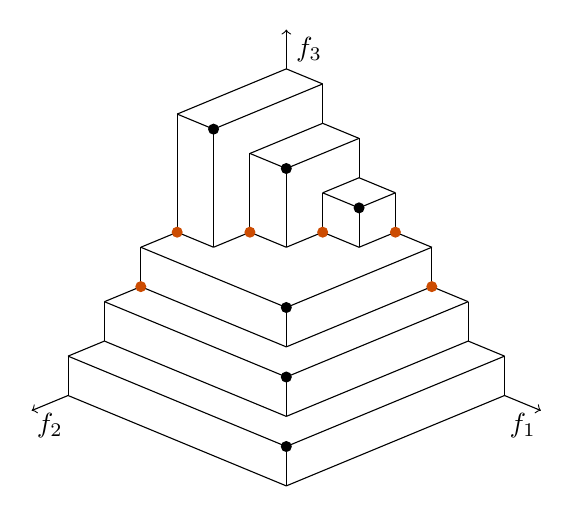
\begin{tikzpicture}
    % lines:
    \draw (-0.9239,2.2346) -- (-1.3858,2.426);
    \draw (-1.3858,2.426) -- (0.0,3.0);
    \draw (-1.3858,2.426) -- (-1.3858,0.926);
    \draw (-0.9239,2.2346) -- (0.4619,2.8087);
    \draw (0.4619,2.8087) -- (0.0,3.0);
    \draw (0.4619,2.8087) -- (0.4619,2.3087);
    \draw (-0.9239,2.2346) -- (-0.9239,0.7346);
    \draw (-0.9239,0.7346) -- (-1.3858,0.926);
    \draw (-0.9239,0.7346) -- (-0.4619,0.926);
    \draw (0.0,1.7346) -- (-0.4619,1.926);
    \draw (-0.4619,1.926) -- (0.4619,2.3087);
    \draw (-0.4619,1.926) -- (-0.4619,0.926);
    \draw (0.0,1.7346) -- (0.9239,2.1173);
    \draw (0.9239,2.1173) -- (0.4619,2.3087);
    \draw (0.9239,2.1173) -- (0.9239,1.6173);
    \draw (0.0,1.7346) -- (0.0,0.7346);
    \draw (0.0,0.7346) -- (-0.4619,0.926);
    \draw (0.0,0.7346) -- (0.4619,0.926);
    \draw (0.9239,1.2346) -- (0.4619,1.426);
    \draw (0.4619,1.426) -- (0.9239,1.6173);
    \draw (0.4619,1.426) -- (0.4619,0.926);
    \draw (0.9239,1.2346) -- (1.3858,1.426);
    \draw (1.3858,1.426) -- (0.9239,1.6173);
    \draw (1.3858,1.426) -- (1.3858,0.926);
    \draw (0.9239,1.2346) -- (0.9239,0.7346);
    \draw (0.9239,0.7346) -- (0.4619,0.926);
    \draw (0.9239,0.7346) -- (1.3858,0.926);
    \draw (0.0,-1.7961) -- (-2.7716,-0.6481);
    \draw (-2.7716,-0.6481) -- (-2.3097,-0.4567);
    \draw (-2.7716,-0.6481) -- (-2.7716,-1.1481);
    \draw (0.0,-1.7961) -- (2.7716,-0.6481);
    \draw (2.7716,-0.6481) -- (2.3097,-0.4567);
    \draw (2.7716,-0.6481) -- (2.7716,-1.1481);
    \draw (0.0,-1.7961) -- (0.0,-2.2961);
    \draw (0.0,-2.2961) -- (-2.7716,-1.1481);
    \draw (0.0,-2.2961) -- (2.7716,-1.1481);
    \draw (0.0,-0.9134) -- (-2.3097,0.0433);
    \draw (-2.3097,0.0433) -- (-1.8478,0.2346);
    \draw (-2.3097,0.0433) -- (-2.3097,-0.4567);
    \draw (0.0,-0.9134) -- (2.3097,0.0433);
    \draw (2.3097,0.0433) -- (1.8478,0.2346);
    \draw (2.3097,0.0433) -- (2.3097,-0.4567);
    \draw (0.0,-0.9134) -- (0.0,-1.4134);
    \draw (0.0,-1.4134) -- (-2.3097,-0.4567);
    \draw (0.0,-1.4134) -- (2.3097,-0.4567);
    \draw (0.0,-0.0307) -- (-1.8478,0.7346);
    \draw (-1.8478,0.7346) -- (-1.3858,0.926);
    \draw (-1.8478,0.7346) -- (-1.8478,0.2346);
    \draw (0.0,-0.0307) -- (1.8478,0.7346);
    \draw (1.8478,0.7346) -- (1.3858,0.926);
    \draw (1.8478,0.7346) -- (1.8478,0.2346);
    \draw (0.0,-0.0307) -- (0.0,-0.5307);
    \draw (0.0,-0.5307) -- (-1.8478,0.2346);
    \draw (0.0,-0.5307) -- (1.8478,0.2346);
    % points:
    \fill[black] (-0.9238795325112866,2.2346331352698203) circle (2pt) ;
    \fill[black] (0.0,1.7346331352698203) circle (2pt) ;
    \fill[black] (0.9238795325112866,1.2346331352698203) circle (2pt) ;
    \fill[black] (0.0,-1.7961005941905386) circle (2pt) ;
    \fill[black] (0.0,-0.913417161825449) circle (2pt) ;
    \fill[black] (0.0,-0.030733729460359127) circle (2pt) ;
    % kink points:
    \fill[nodecol] (-1.38581929876693,0.9259748514523654) circle (2pt) ;
    \fill[nodecol] (-0.46193976625564337,0.9259748514523654) circle (2pt) ;
    \fill[nodecol] (0.46193976625564337,0.9259748514523654) circle (2pt) ;
    \fill[nodecol] (1.38581929876693,0.9259748514523654) circle (2pt) ;
    \fill[nodecol] (-1.8477590650225735,0.23463313526982044) circle (2pt) ;
    \fill[nodecol] (1.8477590650225735,0.23463313526982044) circle (2pt) ;
    % axes:
    \draw[->] (2.7716,-1.1481) -- (3.2336,-1.3394) node[midway, below] {\( f_1 \)};
    \draw[->] (-2.7716,-1.1481) -- (-3.2336,-1.3394) node[midway, below] {\( f_2 \)};
    \draw[->] (0.0,3.0) -- (0.0,3.5) node[midway, right] {\( f_3 \)};
\end{tikzpicture}
        \caption{Stanje po dodajanju šeste točke.}
        \label{example4d_4}
    \end{subfigure}

    \caption{Vizualizacija stanja $\sp$ po dodajanju točk iz $\P$. S črno barvo so označene točke v $\sp$, z oranžno barvo pa novonastale vpete točke pri dodajanju zadnje točke v $\sp$. Pri dodajanju prvih $\frac{n}{2}$ točk vsakič nastanejo tri nove vpete točke, kot vidimo na sliki~\ref{example4d_1}. Pri dodajanju druge polovice točk, pa vsakič nastane $(\frac{n}{2} + 1) + 2$ novih vpetih točk, kot vidimo na slikah~\ref{example4d_2},~\ref{example4d_3} in~\ref{example4d_4}.}
    \label{fig:example4d}
\end{figure}

Podobno kot za število vpetih točk v štirih dimenzijah, lahko tudi za dimenzije $D > 4$ pokažemo, da je vpetih točk največ $O(n^{D-2})$. Ne vemo pa, ali je ta zgornja meja tesna. Glede na to, da je število vpetih točk v dveh in treh dimenzijah linearno, bi bilo prav tako mogoče, da je vpetih točk $O(n^{\lfloor \frac{D}{2} \rfloor})$. Taka meja se pojavi pri problemu Kleejeve mere~\cite{Bringmann}, torej računanja volumna unije kvadrov vzporednih z koordinatnimi osmi.
\end{dokaz}

\subsubsection{Časovna zahtevnost v treh dimenzijah} 
Najprej si oglejmo algoritem \Call{Vpete točke 3d}{$\P$} (algoritem \ref{alg:vpete_tocke_3d}).
Za inicializacijo struktur $\V$, $\sp$, $\sv$ in $h$ porabimo konstanten čas. Množico $\V$ implementiramo kot seznam, stanji $\sp$ in $\sv$ kot urejen seznam, ki podpira dodajanje in iskanje v logaritemskem času~\cite{sortedcontainers}, $h$ pa kot zgoščevalno funkcijo.

Nato v zanki (vrstice 6--16) $n$-krat izvedemo več ukazov. Funkcija \Call{Odstrani dominirane}{$\sv, \overline{\textbf{p}}$} z bisekcijo poišče prvi ter zadnji dominiran element, nato pa ju odstrani in vrne, skupaj z vsemi elementi seznama vmes. Torej je zahtevnost funkcije enaka $O(\log|\sv| + k)$, kjer je $k$ število dominiranih točk v $\sv$. Ker je vsaka točka iz množice $\sv$ odstranjena le enkrat in bo vseh vpetih točk največ $O(n)$, bo po $n$ iteracijah skupna časovna zahtevnost funkcije enaka $O(n \log n)$. 
Podobno se tudi notranjost naslednje zanke (vrstice 9--10), skozi vse iteracije zunanje zanke, izvede le $O(n)$-krat. Znotraj zanke so vse operacije konstantne, torej je skupna časovna zahtevnost vrstic 8--10, skozi celotno delovanje algoritma, enaka $O(n)$. 
V vrstici 11 stanju $\sp$ dodamo novo točko, kar naredimo v $O(\log|\sp|) = O(\log n)$, saj je stanje $\sp$ vedno manjše od števila točk $n$. 
Prav tako v logaritemskem času izračunamo tudi novi vpeti točki, za izračun potrebujemo le indeks elementa $\overline{\textbf{p}}$ v množici $\sp$, nato pa točki izračunamo s pomočjo sosednjih elementov v seznamu. 
Ker je iskanje in nastavljanje elementa v zgoščevalni funkciji v povprečju konstantno, se tudi vrstice 13--15 izvedejo v konstantnem času, dodajanje v stanje $\sv$ pa zopet porabi $O(\log n)$. Torej za celotno zanko for (vrstice 6--16) algoritem porabi $O(n \log n)$ časa. 
Na koncu le še poskrbimo za preostale točke v $\sv$, za katere pa smo že pokazali, da jih je največ $O(n)$. 

Torej je skupna časovna zahtevnost algoritma za iskanje vpetih točk v treh dimenzijah (ter potem tudi algoritma ARRNO v treh dimenzijah) $O(n \log n)$.

\subsubsection{Časovna zahtevnost v višjih dimenzijah}
Naj bo $T(n, D)$ čas, ki ga porabi algoritem za vhodno množico $|\P| = n$ in dimenzijo $D$. Pokazali smo že, da je $T(n, 3) = O(n \log n)$, zdaj pa bi radi izračunali $T(n, D)$ še za poljubno dimenzijo $D > 3$.

Tudi v višjih dimenzijah za inicializacijo stanj potrebujemo konstanten čas, časovno najbolj zahtevne operacije, pa se zgodijo znotraj glavne zanke algoritma \ref{alg:vpete_tocke}. Funkcijo \Call{Odstrani Dominirane}{$\sv, \overline{\textbf{p}}$}, kličemo $n$ krat in potrebuje linearno časovno zahtevnost v odvisnosti od števila točk v $\sv$. Ker je število točk v $\sv$ omejeno z $O(n^{D-2})$, je časovna zahtevnost funkcije v najslabšem primeru $O(n^{D-1})$. Po enakem razmisleku kot v algoritmu treh dimenzij, algoritem za vrstice 10--12 porabi $O(n^{D-2})$ časa. Za dodajanje točke $\overline{\textbf{p}}$ v stanje $\sp$, skupaj z odstranjevanjem dominiranih točk pa je na vsakem koraku potrebno $O(n)$ časa, torej skupaj $O(n^2)$. Računanje novih vpetih točk in dodajanje točk v zgoščevalno funkcijo $h$ v vrsticah 14--17, pa ima znotraj vsake ponovitve časovno zahtevnost $T(n, D-1)$. Za dodajanje preostalih točk iz $\sv$ v $\V(\P)$ pa je potrebno največ $O(n^{D-2})$ časa, kolikor je možnih točk v $\sv$. Torej velja
\[
T(n, D) = O(n^{D-1}) + n T(n, D-1).
\]
Za $D = 4$ torej velja
\[
T(n, 4) = O(n^{3}) + O(n^2 \log n) = O(n^3),
\]
za splošen $D \geq 4$ pa
\[
T(n, D) = O(n^{D-1}).
\]

\subsection{Analiza prostorske zahtevnosti}
Za analizo prostorske zahtevnosti algoritma, spremljamo strukture $\P$ $\V$, $\overline{\V}$, $\sp$, $\sv$ in $h$ tekom algoritma. Vse ostale spremenljivke zasedajo konstantno veliko prostora. Vhodna množica $\P$ je velikosti $O(n)$, kakor tudi stanje $\sp$, ki se inicializira prazno, na koncu pa ima največ $O(n)$ točk. Za izhodno množico vpetih točk smo v trditvi~\ref{sec:st_vpetih_tock} pokazali da vsebuje največ $O(n^{D-2})$ točk, množica $\overline{\V}$ pa $O(n^{D-3})$ točk, saj predstavlja vpete točke problema v nižji dimenziji. Enako kot $\V$ potrebujeta tudi stanje $\sv$ in zgoščevalna funkcija $h$ največ $O(n^{D-2})$ prostora. 

Upoštevati je potrebno tudi prostor, ki ga zasede tudi klicanje rekurzivne funkcije. Znotraj funkcije sicer $n$ krat rekurzivno kličemo funkcijo z nižjo dimenzijo, vendar se hkrati izvaja vedno največ en klic funkcije za vsako dimenzijo $D \geq 3$. Torej je skupna prostorska zahtevnost enaka
\[
\sum_{i=3}^D O(n^{i-2}) = O(n^{D-2}).
\]

\subsection{Eksperimentalna analiza časovne zahtevnosti}
Za ovrednotenje hitrosti algoritma ARRNO izvedemo serijo poskusov pri dimenzijah problema 3, 4, 5 in 6. Testiranje algoritma pri višjih dimenzijah problema je zaradi eksponentne časovne zahtevnosti dolgotrajno, prav tako pa za to tudi ni prave motivacije, saj se z večkriterijsko optimizacijo s tolikšnim številom kriterijev v praksi srečamo redko. 

Testne instance ustvarimo tako, da čim bolj posnemajo scenarij večkriterijske optimizacije, kjer skozi proces optimizacije dobivamo množico paroma nedominiranih točk, ki ji rečemo fronta. Dva primera takih front, ki se pogosto pojavita v raziskavah in se enostavno generalizirata na poljubno število dimenzij sta sferična ter linearna fronta~\cite{Tusar15tevc}. Prav tako pa ustvarimo tudi poseben primer fronte, za katero pričakujemo, da je za algoritem najbolj časovno zahtevna. 

\subsubsection{Linearna fronta}
Linearna fronta je sestavljena iz točk, ki ležijo na hiperravnini v pozitivnem delu koordinatnega sistema in predstavlja primer večkriterijskega problema z linearnim kompromisom med kriteriji. Primera front v dveh in treh dimenzijah vidimo na sliki~\ref{fig:linear_front}.

\begin{figure}[th]
    \centering
    \begin{subfigure}{0.45\textwidth}
        \centering
        \begin{tikzpicture}
  \begin{axis}[
    xlabel={$f_1$},
    ylabel={$f_2$},
    xmin=0, xmax=3.5,
    ymin=0, ymax=3.5,
    width=6cm,
    height=6cm,
    enlargelimits=true,
    axis lines=middle,
    ticks=none
  ]
    \addplot[
      only marks,
      mark=*,
      Greens-I
    ] table [x=x, y=y, col sep=comma] {csv/points_linear_2D.csv};

  \addplot[Greens-F, line width=2pt] coordinates {(0,3) (3,0)};
  
  \end{axis}
\end{tikzpicture}

        \caption{Primer linearne fronte z 20 točkami v dveh dimenzijah.}
        \label{fig:front_linear_2d}
    \end{subfigure}
    \hfill
    \begin{subfigure}{0.45\textwidth}
        \centering
        \begin{tikzpicture}
  \begin{axis}[
    view={100}{25},
    xlabel={$f_2$},
    ylabel={$f_1$},
    zlabel={$f_3$},
    xmin=0, xmax=3.5,
    ymin=0, ymax=3.5,
    zmin=0, zmax=3.5,
    width=7cm,
    height=7cm,
    axis lines=center,
    ticks=none,
    enlargelimits=true
  ]
    \addplot3[
      only marks,
      mark=*,
      Greens-I,
    ] table [x=x, y=y, z=z, col sep=comma] {csv/points_linear_3D.csv};

    \addplot3[
      fill=Greens-F,
      opacity=0.5,
      draw=none
    ]
    coordinates {
      (3,0,0)
      (0,3,0)
      (0,0,3)
    };
    \end{axis}
\end{tikzpicture}
        \caption{Primer linearne fronte z 200 točkami v treh dimenzijah.}
        \label{fig:front_linear_3d}
    \end{subfigure}
    \caption{Primera linearne fronte v dveh dimenzijah na levi in treh dimenzijah na desni.}
    \label{fig:linear_front}
\end{figure}

\subsubsection{Sferična fronta}
Sferična fronta je sestavljena iz točk, ki ležijo na sferi s središčem v izhodišču. Primera front v dveh in treh dimenzijah vidimo na sliki~\ref{fig:spherical_front}.
\begin{figure}[th]
    \begin{subfigure}{0.45\textwidth}
        \centering
        \begin{tikzpicture}
    % lines:
    % points:
    \fill[black] (2.955922741537514,0.5123677839807521) circle (2pt) node[below left] {\(  \)};
    \fill[black] (0.7024754457057101,2.9165953178630324) circle (2pt) node[below left] {\(  \)};
    \fill[black] (1.4078852677873321,2.649124208629598) circle (2pt) node[below left] {\(  \)};
    \fill[black] (2.3646736536199002,1.8461631866863537) circle (2pt) node[below left] {\(  \)};
    \fill[black] (0.36091630696924404,2.9782107748384234) circle (2pt) node[below left] {\(  \)};
    \fill[black] (2.939542845805237,0.5992393993015204) circle (2pt) node[below left] {\(  \)};
    \fill[black] (1.4627203906675144,2.6192458950479383) circle (2pt) node[below left] {\(  \)};
    \fill[black] (2.944601085129371,0.5738679721459727) circle (2pt) node[below left] {\(  \)};
    \fill[black] (1.708883984822526,2.4657079158767132) circle (2pt) node[below left] {\(  \)};
    \fill[black] (1.1239446014177226,2.781501129416265) circle (2pt) node[below left] {\(  \)};
    \fill[black] (2.7334448184804945,1.236235990546359) circle (2pt) node[below left] {\(  \)};
    \fill[black] (1.8317210481023745,2.3758783642978734) circle (2pt) node[below left] {\(  \)};
    \fill[black] (0.12340126135666472,2.9974609469842277) circle (2pt) node[below left] {\(  \)};
    \fill[black] (2.7548787887496924,1.1877048704526834) circle (2pt) node[below left] {\(  \)};
    \fill[black] (1.2757441511913112,2.715230535461245) circle (2pt) node[below left] {\(  \)};
    \fill[black] (1.480712173654873,2.609116988329627) circle (2pt) node[below left] {\(  \)};
    \fill[black] (0.5111149858255252,2.956139623100467) circle (2pt) node[below left] {\(  \)};
    \fill[black] (2.5082062737879474,1.6458740195199573) circle (2pt) node[below left] {\(  \)};
    \fill[black] (2.512050452993866,1.640000768784367) circle (2pt) node[below left] {\(  \)};
    \fill[black] (2.540505618857944,1.5955661066064342) circle (2pt) node[below left] {\(  \)};
    % axes:
    \draw[->] (0,0) -- (4,0) node[midway, below] {\( f_1 \)};
    \draw[->] (0,0) -- (0,4) node[midway, left] {\( f_2 \)};
\end{tikzpicture}
        \caption{Primer sferične fronte z 20 točkami v dveh dimenzijah.}
        \label{fig:front_spherical_2d}
    \end{subfigure}
    \hfill
    \begin{subfigure}{0.45\textwidth}
        \centering
        \begin{tikzpicture}
  \begin{axis}[
    view={100}{25},
    xlabel={$f_2$},
    ylabel={$f_1$},
    zlabel={$f_3$},
    xmin=0, xmax=3.5,
    ymin=0, ymax=3.5,
    zmin=0, zmax=3.5,
    width=7cm,
    height=7cm,
    axis lines=center,
    ticks=none,
    enlargelimits=true
  ]
    \addplot3[
      only marks,
      mark=*,
      Blues-I,
    ] table [x=x, y=y, z=z, col sep=comma] {csv/points_spherical_3D.csv};

    % Approximate positive octant of unit sphere with filled patches
    \foreach \theta in {0,10,...,80} {
      \addplot3[
        fill=Blues-F,
        opacity=0.5,
        draw=none
      ]
      coordinates {
        (0,0,0)
        ({3 * cos(\theta)}, {3 * sin(\theta)}, 0)
        ({3 * cos(\theta+10)}, {3 * sin(\theta+10)}, 0)
      };
    }

    % Same idea: fill along vertical arcs up to z=1
    \foreach \phi in {0,10,...,80} {
      \addplot3[
        fill=Blues-F,
        opacity=0.5,
        draw=none
      ]
      coordinates {
        (0,0,0)
        ({3*cos(0)*cos(\phi)}, {3*sin(0)*cos(\phi)}, {3*sin(\phi)})
        ({3*cos(0)*cos(\phi+10)}, {3*sin(0)*cos(\phi+10)}, {3*sin(\phi+10)})
      };
    }  
    
    % Approximate positive octant of unit sphere with filled patches
    \foreach \theta in {0,10,...,80} {
      \addplot3[
        fill=Blues-F,
        opacity=0.5,
        draw=none
      ]
      coordinates {
        (0,0,0)
        (0, {3 * cos(\theta)}, {3 * sin(\theta)})
        (0, {3 * cos(\theta+10)}, {3 * sin(\theta+10)})
      };
    }
    \end{axis}
\end{tikzpicture}
        \caption{Primer sferične fronte z 200 točkami v treh dimenzijah.}
        \label{fig:front_spherical_3d}
    \end{subfigure}
    \caption{Primera sferične fronte v dveh dimenzijah na levi in treh dimenzijah na desni.}
    \label{fig:spherical_front}
\end{figure}

\subsubsection{Algoritmično zahtevna fronta} 
Za testiranje ustvarimo tudi fronto, za katero velja, da je projekcija točk na prvih $D-1$ koordinat paroma nedominiranih. Intuicija, zakaj naj bi bila taka fronta najtežja za algoritem, je, da bosta imeli stanji $\sp$ in $\sv$ tekom delovanja algoritma vedno več točk. Sestavimo jo tako, da točkam iz linearne fronte z eno manjšo dimenzijo dodamo naključno zadnjo koordinato. Taka definicija je smiselna le za $D \geq 3$, saj množica enodimenzionalnih točk ne more biti paroma nedominiranih. Primer fronte v treh dimenzijah vidimo na sliki~\ref{fig:front_worst_case}.
\begin{figure}[th]
    \centering
    \begin{tikzpicture}
  \begin{axis}[
    view={100}{25},
    xlabel={$f_2$},
    ylabel={$f_1$},
    zlabel={$f_3$},
    xmin=0, xmax=3.5,
    ymin=0, ymax=3.5,
    zmin=0, zmax=3.5,
    width=7cm,
    height=7cm,
    axis lines=center,
    ticks=none,
    enlargelimits=true
  ]
    \addplot3[
      only marks,
      mark=*,
      Reds-I,
    ] table [x=x, y=y, z=z, col sep=comma] {csv/points_worst_case_3D.csv};

    \addplot3[
      fill=Reds-F,
      opacity=0.5,
      draw=none
    ]
    coordinates {
      (3,0,0)
      (0,3,0)
      (0,3,3)
      (3,0,3)
    };

  \end{axis}
\end{tikzpicture}
    \caption{Primer algoritmično zahtevne fronte z 200 točkami v treh dimenzijah.}
    \label{fig:front_worst_case}
\end{figure}


\subsubsection{Okolje poskusov}
Algoritem implementiramo v programskem jeziku Python 3.10. Poskuse izvedemo na računalniku z operacijskim sistemom Windows z 2,40 GHz procesorjem Intel Core i7-12800H s 14 jedri in 32 GB pomnilnika RAM.

\subsubsection{Rezultati poskusov}
Algoritem testiramo na linearni in sferični fronti v dimenzijah 3, 4, 5 in 6. Za naključno ustvarjeno fronto $\P$ in naključno izbrano točko $\textbf{q} \succeq 0$, $\textbf{q} \notin N(\P)$, merimo čas, ki ga algoritem porabi za izračun razdalje do nedominiranega območja. Začnemo z množico $\P$, ki vsebuje le eno točko, nato pa velikost množice podvajamo, dokler algoritem za računanje ne porabi več kot 60 sekund. Pri vsaki velikosti množice $\P$ eksperiment ponovimo desetkrat, vsakič z novo fronto in novo točko, da dobimo čim bolj robustno oceno časovne zahtevnosti. 
\begin{figure}[htb]
    \centering
    \begin{tikzpicture}
\begin{loglogaxis}[
    width=11.5cm,
    height=8cm,
    grid=major,
    grid style={dashed, gray!25},
    minor tick num=0,
    title={Povprečna hitrost algoritma pri različnih dimenzijah in oblikah fronte},
    xlabel={$|\P|$},
    ylabel={Čas [s]},
    legend style={at={(1.05,1)}, anchor=north west},
    legend cell align={left},
    cycle list={
        {Reds-F, very thick, mark=none},
        {Reds-H, very thick, mark=none},
        {Reds-J, very thick, mark=none},
        {Reds-L, very thick, mark=none},
        {Blues-F, very thick, mark=none},
        {Blues-H, very thick, mark=none},
        {Blues-J, very thick, mark=none},
        {Blues-L, very thick, mark=none},
        {Greens-F, very thick, mark=none},
        {Greens-H, very thick, mark=none},
        {Greens-J, very thick, mark=none},
        {Greens-L, very thick, mark=none}
    }
]

% Plots will automatically cycle through the defined colors
\addplot table [x=front_size, y=mean, col sep=comma] {csv/time_worst_case_3D_1.csv};
\addlegendentry{zah 3D}

\addplot table [x=front_size, y=mean, col sep=comma] {csv/time_worst_case_4D_1.csv};
\addlegendentry{zah 4D}

\addplot table [x=front_size, y=mean, col sep=comma] {csv/time_worst_case_5D_1.csv};
\addlegendentry{zah 5D}

\addplot table [x=front_size, y=mean, col sep=comma] {csv/time_worst_case_6D_1.csv};
\addlegendentry{zah 6D}

\addplot table [x=front_size, y=mean, col sep=comma] {csv/time_spherical_3D_1.csv};
\addlegendentry{sfer 3D}

\addplot table [x=front_size, y=mean, col sep=comma] {csv/time_spherical_4D_1.csv};
\addlegendentry{sfer 4D}

\addplot table [x=front_size, y=mean, col sep=comma] {csv/time_spherical_5D_1.csv};
\addlegendentry{sfer 5D}

\addplot table [x=front_size, y=mean, col sep=comma] {csv/time_spherical_6D_1.csv};
\addlegendentry{sfer 6D}

\addplot table [x=front_size, y=mean, col sep=comma] {csv/time_linear_3D_1.csv};
\addlegendentry{lin 3D}

\addplot table [x=front_size, y=mean, col sep=comma] {csv/time_linear_4D_1.csv};
\addlegendentry{lin 4D}

\addplot table [x=front_size, y=mean, col sep=comma] {csv/time_linear_5D_1.csv};
\addlegendentry{lin 5D}

\addplot table [x=front_size, y=mean, col sep=comma] {csv/time_linear_6D_1.csv};
\addlegendentry{lin 6D}



\end{loglogaxis}
\end{tikzpicture}
    \caption{Graf prikazuje hitrost algoritma v odvisnosti od velikosti množice $\P$. Z odtenki rdeče barve so prikazani povprečni časi testiranja na zahtevni fronti, z odtenki modre povprečni časi na sferični fronti, z odtenki zelene pa časi na linearni fronti. Rezultati so prikazani za fronte od dimenzije 3 z najsvetlejšim odtenkom, do fronte dimenzije 6 z najtemnejšim odtenkom.}
    \label{fig:performance}
\end{figure}

Rezultate prikažemo na sliki~\ref{fig:performance}. Opazimo, da algoritem, posebno na problemih v treh in štirih dimenzijah, deluje počasneje za zahtevno fronto kot za linearno ter sferično fronto. Prav tako je očitno, da se z višjo dimenzijo zahtevnost problema veča. Vidimo, da algoritem na problemu v treh dimenzijah deluje zelo hitro, predvsem za linearno in sferično fronto. Tudi algoritem za reševanje problema v štirih dimenzijah deluje razmeroma hitro in je v praksi uporaben za množice do okrog 1000 točk. Za računanje razdalje v petih ali šestih dimenzijah pa algoritem že pri množici $\P$ s sto točkami potrebuje nekaj sekund. Za množice z več točkami ali višje dimenzije pa bi algoritem verjetno potreboval že več minut časa. 

Do zdaj smo obravnavali primer računanja razdalje ene točke $\textbf{q}$ do nedominiranega območja $N(\P)$. Vendar pa je motivacija za algoritem ARRNO v uporabi za urejanje dominiranih rešitev pri algoritmu COMO-CMA-ES, kjer računamo razdaljo za več dominiranih točk $\textbf{q}_1, \dots, \textbf{q}_m$ do nedominiranega območja $N(\P)$ naenkrat. V tem primeru lahko vpete točke izračunamo le enkrat, za vsako točko $\textbf{q}$ pa izračunamo le razdaljo do vseh stožcev definiranih z vpetimi točkami. Zato poskuse ponovimo še enkrat, le da tokrat računamo razdaljo za množice poizvedbenih točk velikosti 10 in 100. Porabljen čas algoritma primerjamo s časom porabljenim za eno točko in rezultate prikažemo na sliki~\ref{fig:performance_mulitple}. 
\begin{figure}[htb]
    \centering
    \begin{subfigure}{0.49\textwidth}
        \centering
        \begin{tikzpicture}
\begin{semilogxaxis}[
    width=7.35cm,
    height=5.0cm,
    grid=major,
    grid style={dashed, gray!20},
    minor tick num=0,
    xlabel={$|\P|$},
    ylabel={Količnik},
    title={Razmerja hitrosti algoritma (3D)},
    legend columns=3,
    legend to name=plots:sharedlegend,
    legend style={
        draw=black,
        fill=white,
        font=\scriptsize,
        column sep=1ex,
        legend columns=3,
        /tikz/every even column/.append style={column sep=1ex},
        at={(0.5,-0.3)},
        anchor=north
    },
    tick label style={font=\scriptsize},
    label style={font=\scriptsize},
    title style={font=\scriptsize},
    cycle list={
        {Reds-G, very thick, mark=none},
        {Blues-G, very thick, mark=none},
        {Greens-G, very thick, mark=none},
        {Reds-K, very thick, mark=none},
        {Blues-K, very thick, mark=none},
        {Greens-K, very thick, mark=none}
    },
]

\addplot table [x=front_size, y=multiplier, col sep=comma] {csv/comparison_worst_case_3D_10.csv};
\addlegendentry{zah 10}

\addplot table [x=front_size, y=multiplier, col sep=comma] {csv/comparison_linear_3D_10.csv};
\addlegendentry{lin 10}

\addplot table [x=front_size, y=multiplier, col sep=comma] {csv/comparison_spherical_3D_10.csv};
\addlegendentry{sfer 10}

\addplot table [x=front_size, y=multiplier, col sep=comma] {csv/comparison_worst_case_3D_100.csv};
\addlegendentry{zah 100}

\addplot table [x=front_size, y=multiplier, col sep=comma] {csv/comparison_linear_3D_100.csv};
\addlegendentry{lin 100}

\addplot table [x=front_size, y=multiplier, col sep=comma] {csv/comparison_spherical_3D_100.csv};
\addlegendentry{sfer 100}

\draw[dotted] (1,1) -- (1000000,1);

\end{semilogxaxis}
\end{tikzpicture}

        %\caption{caption 1}
        %\label{fig:performance_3D}
    \end{subfigure}
    \hfill
    \begin{subfigure}{0.49\textwidth}
        \centering
        \begin{tikzpicture}
\begin{semilogxaxis}[
    width=7.35cm,
    height=5.0cm,
    grid=major,
    grid style={dashed, gray!20},
    minor tick num=0,
    xlabel={$|\P|$},
    ylabel={Količnik},
    title={Razmerja hitrosti algoritma (4D)},
    tick label style={font=\scriptsize},
    label style={font=\scriptsize},
    title style={font=\scriptsize},
    cycle list={
        {Reds-G, very thick, mark=none},
        {Blues-G, very thick, mark=none},
        {Greens-G, very thick, mark=none},
        {Reds-K, very thick, mark=none},
        {Blues-K, very thick, mark=none},
        {Greens-K, very thick, mark=none}
    },
]

\addplot table [x=front_size, y=multiplier, col sep=comma] {csv/comparison_worst_case_4D_10.csv};

\addplot table [x=front_size, y=multiplier, col sep=comma] {csv/comparison_linear_4D_10.csv};

\addplot table [x=front_size, y=multiplier, col sep=comma] {csv/comparison_spherical_4D_10.csv};

\addplot table [x=front_size, y=multiplier, col sep=comma] {csv/comparison_worst_case_4D_100.csv};

\addplot table [x=front_size, y=multiplier, col sep=comma] {csv/comparison_linear_4D_100.csv};

\addplot table [x=front_size, y=multiplier, col sep=comma] {csv/comparison_spherical_4D_100.csv};

\draw[dotted] (1,1) -- (1000000,1);
  
  
\end{semilogxaxis}
\end{tikzpicture}
 
        %\caption{caption 2}
        %\label{fig:performance_4D}
    \end{subfigure}

    \vspace{0.5cm}

    \begin{subfigure}{0.49\textwidth}
        \centering
        \begin{tikzpicture}
\begin{semilogxaxis}[
    width=7.35cm,
    height=5.0cm,
    grid=major,
    grid style={dashed, gray!20},
    minor tick num=0,
    xlabel={$|\P|$},
    ylabel={Količnik},
    title={Razmerja hitrosti algoritma (5D)},
    tick label style={font=\scriptsize},
    label style={font=\scriptsize},
    title style={font=\scriptsize},
    cycle list={
        {Reds-G, very thick, mark=none},
        {Blues-G, very thick, mark=none},
        {Greens-G, very thick, mark=none},
        {Reds-K, very thick, mark=none},
        {Blues-K, very thick, mark=none},
        {Greens-K, very thick, mark=none}
    },
]

\addplot table [x=front_size, y=multiplier, col sep=comma] {csv/comparison_worst_case_5D_10.csv};

\addplot table [x=front_size, y=multiplier, col sep=comma] {csv/comparison_linear_5D_10.csv};

\addplot table [x=front_size, y=multiplier, col sep=comma] {csv/comparison_spherical_5D_10.csv};

\addplot table [x=front_size, y=multiplier, col sep=comma] {csv/comparison_worst_case_5D_100.csv};

\addplot table [x=front_size, y=multiplier, col sep=comma] {csv/comparison_linear_5D_100.csv};

\addplot table [x=front_size, y=multiplier, col sep=comma] {csv/comparison_spherical_5D_100.csv};

\draw[dotted] (1,1) -- (1000000,1);


\end{semilogxaxis}
\end{tikzpicture}

        %\caption{caption 1}
        %\label{fig:performance_5D}
    \end{subfigure}
    \hfill
    \begin{subfigure}{0.49\textwidth}
        \centering
        \begin{tikzpicture}
\begin{semilogxaxis}[
    width=7.35cm,
    height=5.0cm,
    grid=major,
    grid style={dashed, gray!20},
    minor tick num=0,
    xlabel={$|\P|$},
    ylabel={Količnik},
    title={Razmerja hitrosti algoritma (6D)},
    tick label style={font=\scriptsize},
    label style={font=\scriptsize},
    title style={font=\scriptsize},
    cycle list={
        {Reds-G, very thick, mark=none},
        {Blues-G, very thick, mark=none},
        {Greens-G, very thick, mark=none},
        {Reds-K, very thick, mark=none},
        {Blues-K, very thick, mark=none},
        {Greens-K, very thick, mark=none}
    },
]

\addplot table [x=front_size, y=multiplier, col sep=comma] {csv/comparison_worst_case_6D_10.csv};

\addplot table [x=front_size, y=multiplier, col sep=comma] {csv/comparison_linear_6D_10.csv};

\addplot table [x=front_size, y=multiplier, col sep=comma] {csv/comparison_spherical_6D_10.csv};

\addplot table [x=front_size, y=multiplier, col sep=comma] {csv/comparison_worst_case_6D_100.csv};

\addplot table [x=front_size, y=multiplier, col sep=comma] {csv/comparison_linear_6D_100.csv};

\addplot table [x=front_size, y=multiplier, col sep=comma] {csv/comparison_spherical_6D_100.csv};

\draw[dotted] (1,1) -- (1000000,1);


\end{semilogxaxis}
\end{tikzpicture}
 
        %\caption{caption 2}
        %\label{fig:performance_6D}
    \end{subfigure}

    % Legend added only once
    \ref{plots:sharedlegend}

    \caption{Grafi prikazujejo kolikokrat počasnejši je čas algoritma, kadar računamo razdaljo za deset poizvedbenih točk (s svetlejšo barvo) oziroma sto poizvedbenih točk (s temnejšo barvo) v primerjavi s časom algoritma za eno dano poizvedbeno točko. Z odtenki rdeče barve so prikazani rezultati na zahtevni fronti, z modrimi odtenki rezultati na linearni fronti, z zelenimi pa na sferični fronti.}
    \label{fig:performance_mulitple}
\end{figure}

\vspace{40pt} % ne znam drugače ...
Na grafih vidimo, da računanje razdalje do desetih oziroma stotih točk, ni desetkrat oziroma stokrat počasnejše kot računanje razdalje do ene točke. Opazimo tudi, da z naraščajočim številom točk v množici $\P$, količnik pada proti ena, torej vedno večji delež zahtevnosti algoritma postaja iskanje vpetih točk in ne računanje razdalje do njih. 



\section{Zaključek}
\label{sec:zakljucek}
V magistrskem delu smo obravnavali problem računanja razdalje do nedominiranega območja, ki je pomemben del algoritma COMO-CMA-ES za reševanje večkriterijskih optimizacijskih problemov. Do sedaj je obstajal zgolj algoritem za računanje razdalje do nedominiranega območja v dveh dimenzijah, v tem delu pa predstavimo nov algoritem, poimenovan ARRNO, ki deluje za poljubno višjo dimenzijo. S tem smo odprli pot za nadaljnji razvoj algoritmov, kot je COMO-CMA-ES, v višjih dimenzijah.

Algoritem ARRNO temelji na obstoječem dvodimenzionalnem algoritmu, kjer avtorji ugotovijo, da je ključno iskanje vpetih točk. Prav tako se poslužuje tehnike rekurzivnega pometanja, kot jih uporabljata algoritma HV3D+ in HV4D+. Algoritem smo implementirali in vključili v odprtokodno knjižnico \texttt{moarchiving}~\cite{moarchiving}.

Pravilnost algoritma smo potrdili s obsežnim testiranjem, ki smo ga podrobno izpeljali. Poleg tega smo teoretično analizirali prostorsko in časovno zahtevnost algoritma, ki znaša $O(n \log n)$ za probleme v treh dimenzijah in $O(n^{D-1})$ za probleme v več dimenzijah, kjer je $n$ velikost vhodne množice $D$ pa dimenzija problema. Teoretično analizo časovne zahtevnosti smo dopolnili tudi s serijo eksperimentov za različne dimenzije, velikosti in oblike množic točk. Rezultati kažejo, da je algoritem ARRNO za tri in štiridimenzionalne probleme učinkovit in primeren za praktično uporabo, sploh za manjše množice točk.

V prihodnje bi bilo smiselno raziskati možnosti nadaljnje optimizacije algoritma ARRNO, predvsem njegove časovne zahtevnosti za probleme v višjih dimenzijah. Morda obstaja hitrejši algoritem za iskanje vpetih točk ali pa način za omejitev števila vpetih točk, ki jih je potrebno izračunati. Prav tako, bi bilo zanimivo raziskati pristop, ki ne bi temeljil na računanju vpetih točk, ampak bi razdaljo poiskali na kak drug način. 

\end{document}
